\documentclass[]{book}
\usepackage{lmodern}
\usepackage{amssymb,amsmath}
\usepackage{ifxetex,ifluatex}
\usepackage{fixltx2e} % provides \textsubscript
\ifnum 0\ifxetex 1\fi\ifluatex 1\fi=0 % if pdftex
  \usepackage[T1]{fontenc}
  \usepackage[utf8]{inputenc}
\else % if luatex or xelatex
  \ifxetex
    \usepackage{mathspec}
  \else
    \usepackage{fontspec}
  \fi
  \defaultfontfeatures{Ligatures=TeX,Scale=MatchLowercase}
\fi
% use upquote if available, for straight quotes in verbatim environments
\IfFileExists{upquote.sty}{\usepackage{upquote}}{}
% use microtype if available
\IfFileExists{microtype.sty}{%
\usepackage{microtype}
\UseMicrotypeSet[protrusion]{basicmath} % disable protrusion for tt fonts
}{}
\usepackage[margin=1in]{geometry}
\usepackage{hyperref}
\hypersetup{unicode=true,
            pdftitle={R to Python},
            pdfborder={0 0 0},
            breaklinks=true}
\urlstyle{same}  % don't use monospace font for urls
\usepackage{natbib}
\bibliographystyle{apalike}
\usepackage{color}
\usepackage{fancyvrb}
\newcommand{\VerbBar}{|}
\newcommand{\VERB}{\Verb[commandchars=\\\{\}]}
\DefineVerbatimEnvironment{Highlighting}{Verbatim}{commandchars=\\\{\}}
% Add ',fontsize=\small' for more characters per line
\usepackage{framed}
\definecolor{shadecolor}{RGB}{248,248,248}
\newenvironment{Shaded}{\begin{snugshade}}{\end{snugshade}}
\newcommand{\KeywordTok}[1]{\textcolor[rgb]{0.13,0.29,0.53}{\textbf{#1}}}
\newcommand{\DataTypeTok}[1]{\textcolor[rgb]{0.13,0.29,0.53}{#1}}
\newcommand{\DecValTok}[1]{\textcolor[rgb]{0.00,0.00,0.81}{#1}}
\newcommand{\BaseNTok}[1]{\textcolor[rgb]{0.00,0.00,0.81}{#1}}
\newcommand{\FloatTok}[1]{\textcolor[rgb]{0.00,0.00,0.81}{#1}}
\newcommand{\ConstantTok}[1]{\textcolor[rgb]{0.00,0.00,0.00}{#1}}
\newcommand{\CharTok}[1]{\textcolor[rgb]{0.31,0.60,0.02}{#1}}
\newcommand{\SpecialCharTok}[1]{\textcolor[rgb]{0.00,0.00,0.00}{#1}}
\newcommand{\StringTok}[1]{\textcolor[rgb]{0.31,0.60,0.02}{#1}}
\newcommand{\VerbatimStringTok}[1]{\textcolor[rgb]{0.31,0.60,0.02}{#1}}
\newcommand{\SpecialStringTok}[1]{\textcolor[rgb]{0.31,0.60,0.02}{#1}}
\newcommand{\ImportTok}[1]{#1}
\newcommand{\CommentTok}[1]{\textcolor[rgb]{0.56,0.35,0.01}{\textit{#1}}}
\newcommand{\DocumentationTok}[1]{\textcolor[rgb]{0.56,0.35,0.01}{\textbf{\textit{#1}}}}
\newcommand{\AnnotationTok}[1]{\textcolor[rgb]{0.56,0.35,0.01}{\textbf{\textit{#1}}}}
\newcommand{\CommentVarTok}[1]{\textcolor[rgb]{0.56,0.35,0.01}{\textbf{\textit{#1}}}}
\newcommand{\OtherTok}[1]{\textcolor[rgb]{0.56,0.35,0.01}{#1}}
\newcommand{\FunctionTok}[1]{\textcolor[rgb]{0.00,0.00,0.00}{#1}}
\newcommand{\VariableTok}[1]{\textcolor[rgb]{0.00,0.00,0.00}{#1}}
\newcommand{\ControlFlowTok}[1]{\textcolor[rgb]{0.13,0.29,0.53}{\textbf{#1}}}
\newcommand{\OperatorTok}[1]{\textcolor[rgb]{0.81,0.36,0.00}{\textbf{#1}}}
\newcommand{\BuiltInTok}[1]{#1}
\newcommand{\ExtensionTok}[1]{#1}
\newcommand{\PreprocessorTok}[1]{\textcolor[rgb]{0.56,0.35,0.01}{\textit{#1}}}
\newcommand{\AttributeTok}[1]{\textcolor[rgb]{0.77,0.63,0.00}{#1}}
\newcommand{\RegionMarkerTok}[1]{#1}
\newcommand{\InformationTok}[1]{\textcolor[rgb]{0.56,0.35,0.01}{\textbf{\textit{#1}}}}
\newcommand{\WarningTok}[1]{\textcolor[rgb]{0.56,0.35,0.01}{\textbf{\textit{#1}}}}
\newcommand{\AlertTok}[1]{\textcolor[rgb]{0.94,0.16,0.16}{#1}}
\newcommand{\ErrorTok}[1]{\textcolor[rgb]{0.64,0.00,0.00}{\textbf{#1}}}
\newcommand{\NormalTok}[1]{#1}
\usepackage{longtable,booktabs}
\usepackage{graphicx,grffile}
\makeatletter
\def\maxwidth{\ifdim\Gin@nat@width>\linewidth\linewidth\else\Gin@nat@width\fi}
\def\maxheight{\ifdim\Gin@nat@height>\textheight\textheight\else\Gin@nat@height\fi}
\makeatother
% Scale images if necessary, so that they will not overflow the page
% margins by default, and it is still possible to overwrite the defaults
% using explicit options in \includegraphics[width, height, ...]{}
\setkeys{Gin}{width=\maxwidth,height=\maxheight,keepaspectratio}
\IfFileExists{parskip.sty}{%
\usepackage{parskip}
}{% else
\setlength{\parindent}{0pt}
\setlength{\parskip}{6pt plus 2pt minus 1pt}
}
\setlength{\emergencystretch}{3em}  % prevent overfull lines
\providecommand{\tightlist}{%
  \setlength{\itemsep}{0pt}\setlength{\parskip}{0pt}}
\setcounter{secnumdepth}{5}
% Redefines (sub)paragraphs to behave more like sections
\ifx\paragraph\undefined\else
\let\oldparagraph\paragraph
\renewcommand{\paragraph}[1]{\oldparagraph{#1}\mbox{}}
\fi
\ifx\subparagraph\undefined\else
\let\oldsubparagraph\subparagraph
\renewcommand{\subparagraph}[1]{\oldsubparagraph{#1}\mbox{}}
\fi

%%% Use protect on footnotes to avoid problems with footnotes in titles
\let\rmarkdownfootnote\footnote%
\def\footnote{\protect\rmarkdownfootnote}

%%% Change title format to be more compact
\usepackage{titling}

% Create subtitle command for use in maketitle
\newcommand{\subtitle}[1]{
  \posttitle{
    \begin{center}\large#1\end{center}
    }
}

\setlength{\droptitle}{-2em}

  \title{R to Python}
    \pretitle{\vspace{\droptitle}\centering\huge}
  \posttitle{\par}
    \author{}
    \preauthor{}\postauthor{}
    \date{}
    \predate{}\postdate{}
  
\usepackage{booktabs}
\usepackage{amsthm}
\usepackage{makeidx}
\makeindex
\makeatletter
\def\thm@space@setup{%
  \thm@preskip=8pt plus 2pt minus 4pt
  \thm@postskip=\thm@preskip
}
\makeatother

\usepackage{amsthm}
\newtheorem{theorem}{Theorem}[chapter]
\newtheorem{lemma}{Lemma}[chapter]
\theoremstyle{definition}
\newtheorem{definition}{Definition}[chapter]
\newtheorem{corollary}{Corollary}[chapter]
\newtheorem{proposition}{Proposition}[chapter]
\theoremstyle{definition}
\newtheorem{example}{Example}[chapter]
\theoremstyle{definition}
\newtheorem{exercise}{Exercise}[chapter]
\theoremstyle{remark}
\newtheorem*{remark}{Remark}
\newtheorem*{solution}{Solution}
\begin{document}
\maketitle

{
\setcounter{tocdepth}{1}
\tableofcontents
}
\part{Thoughts of an R programmer Learning
Python}\label{part-thoughts-of-an-r-programmer-learning-python}

\chapter{Front Material}\label{front-material}

\section{Colophon}\label{colophon}

R to Python

Thoughts of an R programmer Learning Python

\begin{figure}
\centering
\includegraphics{images/Janus-iStock-494706611alpha.png}
\caption{Janus}
\end{figure}

by David A York

Copyright 2018 David A York

\url{http://crunches-data.appspot.com/contact.html}

This manuscript may be freely copied and distributed, under the MIT
Licence

self-published, on Toth-York Imprint, Calhoun GA USA, November 27, 2018

\url{https://github.com/medmatix/RPythonBook}

A \href{RPythonBookc.pdf}{pdf} copy with hapters completed to date is
available.

\begin{center}\rule{0.5\linewidth}{\linethickness}\end{center}

\begin{quote}
``In ancient Roman religion and myth, Janus (/ˈdʒeɪnəs/; Latin: IANVS
(Iānus), pronounced {[}ˈjaː.nus{]}) is the god of beginnings, gates,
transitions, time, duality, doorways,{[}1{]} passages, and endings. He
is usually depicted as having two faces, since he looks to the future
and to the past.''
\end{quote}

\begin{quote}
from Wikipedia, \url{https://en.wikipedia.org/wiki/Janus}, accessed 27
November, 2018 at 4:17PM
\end{quote}

Disclaimer: The opinions in this book are ventured based upon my own
experiences and explorations. Others may have different experiences and
drawn different conclusions. I would be interested in hearing yours. Be
constructive and civil please. Dogma will be burned with the banned
books on Guy Fawkes day.

David York 2018;
email:\href{mailto:rpyfeedback@gmail.com}{\nolinkurl{rpyfeedback@gmail.com}}

\section{Preface}\label{preface}

This book is a work in progress on the thoughts of an R programmer (the
author) moving to (or learning) Python. It is intended as a comparison
of R and Python for those already using R. The hop is to ease the way
for those in particular newer to programming as opposed to the quick
task oriented scripting which R lends itself so well to.

As with any language the most visible presence on line are the hardened
champions of the languages with the pressure to standardization (not a
bad thing per-se) and dogmatic adherence to the ``blah blah'' way of
doing things (which is less desirable I think). For those of us who are
not playing at being computer scientist but just scientists with a need
for tools to do our work mose effectively an approachable treatment of
scripting and programming is helpful. There are better computer science
texts and better programming texts than this book would ever purport to
be. I will often be reminding the reader that this is not a beginning
programming book. Neither is it a Computer Science text book. It is a
book by a applied programmers for applied programmers who operate in
other research domains.

Having started as an R user, then as an R programmer, I have relatively
recently embarked on learning python as well. Why I would do this is
rather complicated to explain, particularly as I had knowledge of other
general programming languages, which would conceivably serve such a
role, particularly BASIC and Java. Suffice to say that as a budding Data
Scientist I see lots of reasons to know both R and Python. BASIC, though
still extant it is very limited in support and relevant libraries by
comparison. Java . . . well, as a strong open source advocate I feel
Java is bound to Oracle in many ways for all time. It is likely they
have no intention of truly releasing it into the public domain, ever.
There is far more rationel to learn C++ these days than Java for the
sake of what is arguably only minor difference in learning curve.

I absolutely love R! When I returned to school to study Applied Math and
Statistics it was an ever present partner for me. It could do most
things I needed, though matrix math was less smooth than Matlab the
price was right (not withstanding Octave or Scilab). However, I
increasingly found the need for a general purpose programming language
and Python was there growing in the guise of `the' data science
alternative.

But while R was great with vectorized functions python, at it's core,
was weak in this regard. The libraries for python have been growing
steadily in number and variety, and the functionality gap between it and
R narrows in cluding for vectorized application. I still cannot see a
Data Scientist being as productive not knowing R at this point. However,
I see no reason not to also know Python - ergo, I think any serious Data
Science needs to know both; AND, there is the added incentive of the
interoperability of R and Python (and C++)! From R we have
\href{https://cran.cnr.berkeley.edu/web/packages/XRPython/index.html}{XRPython}
and
\href{https://cran.cnr.berkeley.edu/web/packages/reticulate/index.html}{reticulate}
and from Python we have \href{https://rpy2.bitbucket.io/}{Rpy2}.

There are far more choices for languages to do Data Science with than I
am dealing with here. Arguably, at time point, R and Python seem the
most suitable overall to ``out of the gate'' data analysis. Julia is
comming on strong, and C++ is everyones speed oriented fall back.
However speed is loosing place in the decision criteria as benchmark
comparisons increasingly are show. Most new packages are written in C or
C++ anyway and Cython makes this fairly approachable for python package
developers. Bottlenecks in Big Data analysis are rarely CPU limited
where out of RAM processing, large files and disk access become the
limiting factors.

The Organization of the book is in 3 parts. A close Comparison and
discussion of R and Python unburdened by a mandate to comprehensively
teach beginning programming in either. The first is the overviews of
part 1, I only touch quite generally on the nature of the usual The
procedural elements of programming structures, Variables, datatypes and
data structures, binary decisions, repeating code blocks are all
internals in declarative or functional programming - they are just
details. The Same can be said for languages introducing object-oriented
programming models.

In the second part of the book, an opportunity is taken to compare how
data science can be done in R and Python in some of the various domains
we work. The distinction between function and object is quite blurred
here.

In part 3, a collection of syntax summaries, library reference materials
and resources are compiled in Appendices.

In a sense one could consider this book as a second or third source for
applied R users \index{learning python} - perhaps after the beginner and
intermediate level courses to get the necessary python syntax vocabulary
and programming structures. (see
\href{references.html\#Lutz-Mark-Learning-\%20Python-4th-Ed-OReilly-Media-Sebastopol-CA-2009}{Learning
Python})

\chapter{Introduction}\label{introduction}

This is not a book on learning to program with R or python. Consider it
the companion for non-programmers who are learning python
\index{learning python}with some knowledge of R.

Learning a new programming or scripting language begs comparison. Often
this is not overly helpful to the learner who, coming from a zone of
comfort is often frustrated by the old subtleties not consciously
recognized, being yet unknown in the new. I recall a family member,
completely new to computers, saying why doesn't it know what I mean
expecting the implied parts of language to transfer from English (or
German, or Chinese etc.) to computer language.

R writers early on recognize the absence of vectorization of functions
in core python. It's available though in numpy and pandas, but base
python doesn't have it and they miss it. You'll get there, really.
Object Orientation is also not natural to either R or Python. It came
later to both, but it seems more smoothly accomplished by python than R.

I soon realized, though that you had to know the programming
commonalities of python first; R comparisons really should start with
the libraries of python. R in someways has cut right to the data science
chase often at the expense of strong programming constructs. This is the
nod to interactive coding and scripting rather than the need to
undertake formal programming. Python began early on with a scripting
functionality but it wasn't until the development of iPython that
interactive python could be realized in the way that R users were used
to.

All this is not to say that R was lacking in basic programming
constructs from the start, it wasn't; but the proportion of users who
used R in a quick-and-dirty small problem focused way was quite high.
This suited it's use as a learning environment for introductory
statistics\textsuperscript{7}. I should think that those who try to
start python at the same time as their first statistics course will find
the \index{learning curve}learning curve too steep to help with their
need to learn statistics.

Dalgaard\textsuperscript{7} \index{Dalgaard} was the first source I used
to learn R during my second semester of Statistics. I similarly used
Lutz\textsuperscript{8} \index{Lutz} to learn Python well after I was
comfortable with R and Probability and Statistics. One needs to get past
the very basic programming knowledge of python to effectively get up to
speed with matrix algebra, probability and statistics and data munging
using the available libraries outside of the basic and Standard
Library\textsuperscript{2} \index{standard library} functions of python.
There are books to help you cut some corners in applying python to data
science\textsuperscript{9,} \textsuperscript{10}, but it's very easy to
find oneself confused without a good level of comfort with the ideas and
the pitfalls of importing modules in python. Namespaces
\index{namespace} and variable visibility are less forgiving in python
than R.

Once you get comfortable with the math and stats functions available in
Numpy \index{numpy} and/or \index{scipy} Scipy modules, the data
structures and munging functions of Pandas \index{Pandas} and the
graphics and plotting functions of \index{matplotlib} Matplotlib you are
up to the speed you had gotten to much earlier with R.

As a final word, it may seem like I distain style, in favor of
substance. I recall in a list of interview questions somewhere whether
software that worked was more important than well documented code or
vis-a-versa. It is a trick question. Though software that doesn't work
is useless, it may be worse if it is unfixable too. You can't debug what
is not understandable and spagetti code that is undocumented and
disappearing into thin air never to be seen again is impossible to work
on. Not only will others who want to adapt or debug our old code be
lost, but given a month away from it, we probably won't know whatwe
mwere doing either. Comment obscessively from the start.

There is a plethora of free open source code and applications out there.
Poor documention for users is lazy and sloppy and betrays our
responsibility to tell our clients how to use the solutions we offer.
Sometimes those clients are us and we deserve better too. Writing user
documentation helps us think about our projects in a new perspective -
making our work more valuable.

Reproducibility is a necessity for any modern endeavor. In the face of
the reseach fraud resurfacing more and more, we can no longer ask people
to ``just trust us''. Data Scientists must know this from the outset.
markdown with integrated code, Rstudio and Jupyter addresses this issue
superbly well and so their use is central to what I am writing. The fact
that they allow multi-language processing in the documents is the bonus.
See the References and Resources at the end of the book for other books
and articles on Documentation, \index{style}Style and Reprpoducibility
\index{Reproducibility}.

So now we can forge ahead and look at R and python side-by-side and
perhaps reduce the learning curve for python \index{Data Science}
DataScience libraries.

\part{R and Python, Side by
Side}\label{part-r-and-python-side-by-side}

\chapter{A Comparative Look}\label{a-comparative-look}

As already mentioned, it is not the intent of this treatise to teach
either beginning R or python scripting. There are many good sources for
this and yet another beginners book or tutorial I believe is not needed.
For ease of reference, I include in the \href{Appendix_1.md}{Appendix1}
an overview of relevant R and python syntax and the general programming
constructs common to any functional language. In Part 1, at the risk of
being pedantic, I am giving a generic overview of the components of the
typical script or program to be used as a framework in organizing our R
and Python comparisons.

\section{Functional Programming
Commonalities.}\label{functional-programming-commonalities.}

In functional programming, a kind of declarative paradigm, operational
code is incorporated by task and purpose into blocks of code which are
called by name in the body of a script. In practice it is most often a
hybride rather than any one pure paradigm incolved. As a result some
connecting statements and assignments in the program of script set up a
milieu in which the functions operate together to accomplish some larger
task.

Historically, Fortran and Basic code in common academic and educational
use, became unwieldy as users became increasingly prone to the writing
of rampant spagetti code. The introduction of the concept of `structured
programming' and the uniform reliance on subroutine and function calls
mostly tamed the spagetti-monster within a procedural programming
paradigm. Growth of functional programming with pascal and to some
extent modern C was a natural evolution of this trend and object
oriented extensions to most legacy languages exist as we'll see later
on.

So the perspective of R and Python as relying on script collections of
functions calling each other is what we are stressing now. Purely
Functional programs use functions and flow is linear through the
collection which makes up the program. In a strict sense this would be
done without regard to flow control, but functions are just in a sense
subprograms with all the statements of procedural tasks and flow control
within, common to the usual conception of programs.

I will deal, in a general way with the, statement types which make up
the functions and include comparsions between how R and Python each
express the tasks. As I've already stressed,this book not aimed at
teaching beginning programming. Consult the bibliography for some
suggested sources for beginning programmers\^{}7, 8\^{}.
\index{beginner programming} \index{learning python}

The later innovation of object oriented programming concepts evolving
from this will be touched on in a comparative fashion in another
chapter.

\section{Building Blocks of Functions as
Procedures}\label{building-blocks-of-functions-as-procedures}

\subsection{\texorpdfstring{Statements and Expressions
\index{statements}
\index{expression}}{Statements and Expressions  }}\label{statements-and-expressions}

A program or script is of course considered as a series of instructions
grouped together and run as a unit. These statements constitute
expressions of mathemetical equations (see specifically \href{}{Chapter
5}), choices, and other orders to be carried out by the machine.

With any program or script statements tasks and values stored are
executed or accessed from memory locations. This was the innovation
conceived of by John Von Neumann which moved programming from the moving
wire jumpers to the input to the machine from various codes punched into
tapes or cards to be held in memory while being used.

\subsection{\texorpdfstring{Assignment of Values to Memory and the
Variable
\index{assignement statements}}{Assignment of Values to Memory and the Variable }}\label{assignment-of-values-to-memory-and-the-variable}

Variables are memory locations assigned values as the computing process
goes on. The classification of specific locations determines a type of
data held there.

The codes stored in the machine include a specific operator code to
direct the move of a value received for input or a statement's result to
a memory location. This is called and assignment.

Traditionally R has used the combined dash-less-than symbols
`-\textgreater{}' for this purpose but the simple equals sign `=' now
also works in this fashion. Python uses the same equals sign for
assignments.

Variables are named in both R and Python and neither may begin with a
digit. There are other restrictions and conventions which are not gone
into here.

\subsection{\texorpdfstring{Decisions and Choices \index{conditionals}
\index{branching} \index{program flow}
\index{choices and decisions}}{Decisions and Choices    }}\label{decisions-and-choices}

As currently implemented all choices by a computer resolve to yes or no
results. Some semblance or the greys we think in are a result of a
collection or range of yes-no questions. These choices are explicit or
implicit `if' queries.

\subsection{\texorpdfstring{Doing it Over Again (and again \ldots{})
\index{loops}}{Doing it Over Again (and again \ldots{}) }}\label{doing-it-over-again-and-again}

Loops are created within a program logic, usually involving a choice
test to be executed which cause tasks to be repeated zero or more times.
It is considered bad parctice to create a loop without some form of exit
(short of having to power down the machine).

\subsection{\texorpdfstring{Functions
\index{functions}}{Functions }}\label{functions}

Functions in fortran were short program clips that did a task and
immediately returned a value . Subroutines are more like what functions
in R and Python are, though returning to the calling place with some
value is a frequent option with these functions as well. Functions may
provide a new programming element like a square root (python,
math.sqrt(x)) extending the language, or functions may carry out a whole
task like carring out a liner regression, storing objects of the answer
in memory for retrieval, or return as an object explicitly. Often a
function is called that builds a whole graphic plot for display or other
output when called.

In R,

\begin{verbatim}
function.name <- function(arguments) 
{
    computations on the arguments
    maybe other code too
}
\end{verbatim}

and in Python indents take the place of brackets to define code blocks.
\index{Self} in the function spec is the calling code block, and if
omitted, is created by python implicitly. In the functional paradigm,
\index{self} is always present but implicitly. It becomes important in
object-oriented programming in python where, your first argument
implicitly or explicitly is the calling \index{namespace}.
`\index{Self}' in the indented code block would be the function itself.

\begin{verbatim}

def aroutine(args):
    computations on args
    maybe other code too
  
\end{verbatim}

The notation of R is C (and Java) - like with bracketed blocks, and
Python is Pascal-like with indented blocks. Unlike pascal there is no
`begin:' keyword required to start the script but when named code blocks
are used such as functions the colon is needed at the end of definition.

Functional programming with R and Python, will be expanded on in
\href{06-Functional_Programming.Rmd}{Chapter 6} later on.

\subsection{\texorpdfstring{Objects and Classes anticipating
Object-Oriented Programming
\index{object, class and instance}}{Objects and Classes anticipating Object-Oriented Programming }}\label{objects-and-classes-anticipating-object-oriented-programming}

In general terms we will come to consider all program elements as
objects. A Class will be considered as a pattern definition for an
object in the same fashion as a function definition. All objects are
used as instances of some previously defined class created by an
assignment statement.

\begin{verbatim}

AnInstance=ClassName() # call ClassName constructor to create an instance "AnInstance"

\end{verbatim}

More later in \href{12-OO_Programming.Rmd}{Chapter 12}

\chapter{Set-up for R and Python
Exercises}\label{set-up-for-r-and-python-exercises}

Clearly you have to get R and python onto your system. I have a bias
about dependance on any en block installed software stacks, like
Anaconda etc. Anaconda is a convenient way to install programs together.
However it is easy to loose locations of programs and tools and have
conflicts with installs from outside of the group installers, such as
different Python destributions, and difficult to manage path complexity.

Just the same, Anaconda is a good choice if you are doing a clean
install and intend to do everthing inside that framework.Then installing
\href{https://www.anaconda.com/}{Anaconda,Python Data Science Platform}
can make things much easier in the long run for integrating R and Python
and Reproducible Research work.

All of these sites will help you approach installs and configurations in
a variety of ways. As an R programmer, first I installed
\href{https://www.r-project.org/}{R}, then
\href{https://www.rstudio.com/}{RStudio\textsuperscript{4}}. Once
installed, RStudio is a convenient way to install the R packages as
well.

Then I installed Python 3 from \href{https://www.python.org/}{Python
Software Foundation}. From that point on I used PIP package manager for
python and RGUI for package installs for python and R respectively and
install jupyter see \href{http://jupyter.org/install}{Project
Jupyter}.\index{Project Jupyter} This gave the maximum flexibility for R
and Python in their own environments. I also installed the Scipy
\index{SciPy} (which includes numpy \index{numpy}, and Matplotlib
\index{Matplotlib} all using PIP.

I did do a parallel Anaconda \index{Anaconda} install afterwards with R
and RStudio \index{RStudio} and iPython \index{iPython} for Jupyter
Notebooks but as mentioned there was some path confusion with this
approach. It does set you up nicely for any approach to data science and
development you could choose down the road.

You really are going to need an IDE for Python.
\href{https://www.spyder-ide.org/}{Spyder} \index{Spyder}, available
separately installed with PIP, or installed through Anaconda. It is a
solid python focused choice. I personally use
\href{https://www.eclipse.org/}{Eclipse} \index{Eclipse}as it is open
sourced and you can use it for multiple languages including R (not as
strong yet) and python, HTML/CSS/javascript, C/C++, Java and others.

\section{Package Libraries}\label{package-libraries}

The strength of both R and Python is from their libraries.
\href{https://cran.cnr.berkeley.edu/index.html}{CRAN Package Repository}
\index{CRAN}and \href{http://www.bioconductor.org/about/}{Bioconductor}
\index{Bioconductor} are both well stocked with general and special
purposed functions for R. RStudio develops
\href{https://www.rstudio.com/products/rpackages/}{R Packages}
integrating well with the RStudio environment. The are lost of R
packages in development awaiting addition to CRAN or hosted outside of
CRAN such as on \href{https://github.com/search?q=R+language}{Github}
\index{R on Github}.

If the reader has spent any time with R at all you have likely made
inroads into these package sources. So how does Python compare? Python
comes with a large standard library providing ``out of the gate''
functionality to compare with R-core. The best handing of the
intricacies of the python standard library I've found is Doug Helmann's
\href{https://amazon.com/Python-Standard-Library-Example-Developers/dp/0134291050/}{The
Python 3 Standard Library by example}. Python Software foundation hosts
the \href{https://pypi.org/}{Python Package Index , PyPi} \index{PyPi}
analygous to the CRAN repositories and \index{Bioconnector}. Also, the
most important resource to get you up to speed is
\href{https://www.scipy.org/}{SciPy tools} consisting of SciPy, Numpy,
Pandas and Matplotlib. These are the essential minimum to do any R-like
work in python. These and more can be accessed as well through the
\href{https://numfocus.org/sponsored-projects}{Numfocus Projects}.
\index{Numfocus} Finally, you should check out the
\href{https://www.statsmodels.org/stable/index.html}{StatsModels\textsuperscript{11}}
\index{StatsModels} package site.

\section{Pulling it Together}\label{pulling-it-together}

Having apprised ourselves of the breadth and availability of these
resources we will go forward and organize some of the ideas. R packages
can be installed with the R GUI but the RStudio environment is much
easier for this. Once a package is installed it is available in all
environments I've alluded to. Compiling and installing is always best
and I thing RStudio makes this fairly painless. Remember to start the
GUI, Anaconda or RStudio environment as administrator to keep things
together.

\subsection{The Prompts}\label{the-prompts}

When accessing the R and Python interpreters from the command shell (or
bash) prompt,

\begin{verbatim}
$
\end{verbatim}

after the version and copyright banners, if present, you are at an
interpreter prompt. For R this is:

\begin{verbatim}
>
\end{verbatim}

for python,

\begin{verbatim}
>>>
\end{verbatim}

for iPython

\begin{verbatim}
In [1]:
\end{verbatim}

from this point you enter what ever commands or statements you wish to
execute. These are executed immediately, or continued with continuation
prompts until executable. Once executed any declarations and output are
retained if the were assigned to some object to be held in memory.
Immediate answers are generally lost.

Otherwise, one groups statements into a file to be read all at once and
executed as a group. Objects created are again retained in memory by
default. This is a script of program. Script file extensions are
standardized for the operating system to recognize, eg.(.R for R, and
.py or pyc for python). Python scripts intended to be called by other
scripts for library code to be incorporated are called modules and end
in the same .py extension. A package can be considered, in both R and
python) as a collection of declarations, functions, classes, or modules
for library purposes.

\subsection{\texorpdfstring{Installing Packages
\index{Installing R Packages}}{Installing Packages }}\label{installing-packages}

From the R GUI prompt we have \index{package-install()},

\begin{verbatim}
  package-install()
\end{verbatim}

Python packages from any source mentioned above can be installed with
the PIP utility. This can be done from the shell prompt (remember to
start as administrator or root) \index{installing with PIP}:

\begin{verbatim}

  $ pip install matplotlib  
    # OR
  $ python -m pip install matplotlib
\end{verbatim}

This can be done as root with the anaconda prompt as well.

\subsection{Using Packages}\label{using-packages}

In R we must make sure the package (once installed) is loaded for our
session. This is done with the library() function,

\begin{Shaded}
\begin{Highlighting}[]
  \KeywordTok{library}\NormalTok{(}\StringTok{"reticulate"}\NormalTok{)}
\end{Highlighting}
\end{Shaded}

while in python we import the package previously installed as,

\begin{verbatim}
  import numpy
\end{verbatim}

Once imported or loaded into either, we can access the functions of
reticulate directly by name. If we have a previous function of the same
name it gets overwritten unless in python we keep the name spaces
separate. This can be done by the form of the import statement. We can
also import only slected functions from a package module.

\begin{verbatim}

  import numpy as np             # usual format to use \index{namespace} segregation of functions
  from numpy import sum, matrix  # economical import,still can conflict without renaming 
                                 #   using 'as', such as where base python has a sum()  
                                 #   function and math has a different one called sum()
\end{verbatim}

\section{Using R and Python Together}\label{using-r-and-python-together}

There are several ways that one could find helpful to use R and Python
together, to take best advantage of their respective strengths

\subsection{Working in R and Calling
Python}\label{working-in-r-and-calling-python}

In this instance one would find working in R the necessary starting
place loading the reticulate \index{reticulate} library when finding the
need to employ python functions or packages as helpful to your needs. A
call would be made to the python function from R to have a task
completed by python and control returned to the R program.

\begin{Shaded}
\begin{Highlighting}[]
\KeywordTok{cat}\NormalTok{(}\StringTok{"PI in R is"}\NormalTok{, pi)}
\end{Highlighting}
\end{Shaded}

\begin{verbatim}
## PI in R is 3.141593
\end{verbatim}

\begin{Shaded}
\begin{Highlighting}[]
\ImportTok{import}\NormalTok{ math}
\BuiltInTok{print}\NormalTok{(math.pi)}
\end{Highlighting}
\end{Shaded}

\begin{verbatim}
## 3.141592653589793
\end{verbatim}

\subsection{Working in Python and Calling
R}\label{working-in-python-and-calling-r}

Working in python and calling an R object requires the rpy2 \index{rpy2}
package and would look like,

\begin{verbatim}
# Accessing an R object from from python 
# (example from: http://rpy.sourceforge.net/rpy2/doc-dev/html/introduction.html)
import rpy2.robjects as robjects
rpi = robjects.r['pi']
print("PI from R = ", rpi)
\end{verbatim}

\subsection{Working in Jupyter and Writing in R, Python or Both in the
Same
Notebook}\label{working-in-jupyter-and-writing-in-r-python-or-both-in-the-same-notebook}

There are multiple kernel plugins available for jupyter notebooks. As A
rule, the notebooks only use one language kernel at a time. An exception
is the {[}SOS kernel{]}(\url{https://vatlab.github.io/sos-docs/}.

Jupyter is running first level in python. It is afterall a python
module. When running the R kernel (irkernel)\index{irkernel} remember
you are running R in python. See the caution below in the contest of
rMarkdown code chunks.

Consider this Jupyter notebook using the R kernel,

\begin{figure}
\centering
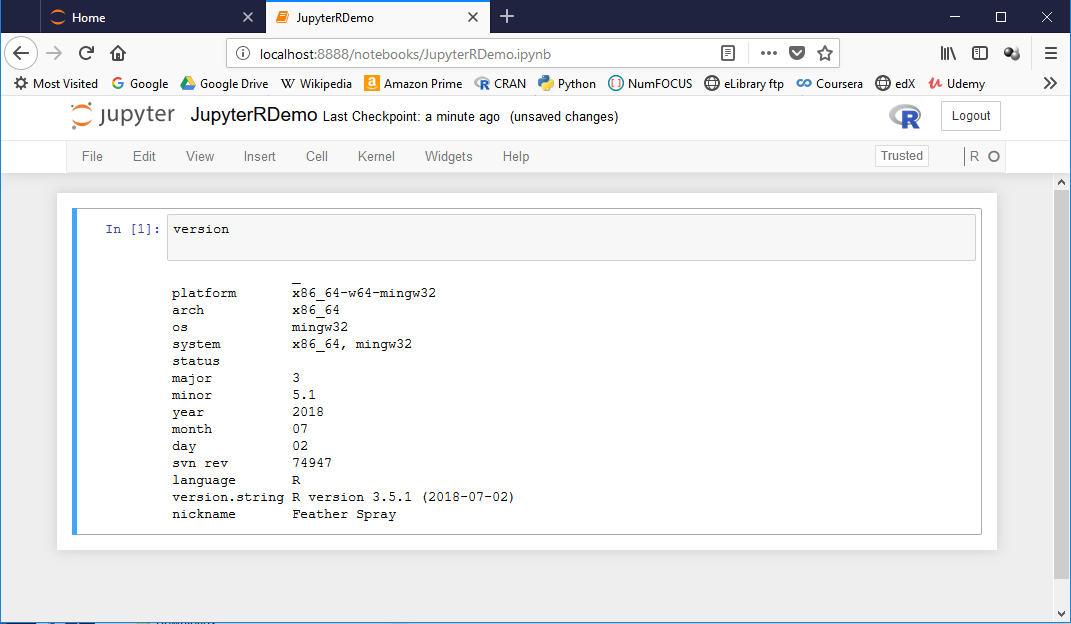
\includegraphics{images/JupyterRSession.png}
\caption{Jupyter R Demo}
\end{figure}

and this Jupyter notebook using the `Python kernel',

\begin{figure}
\centering
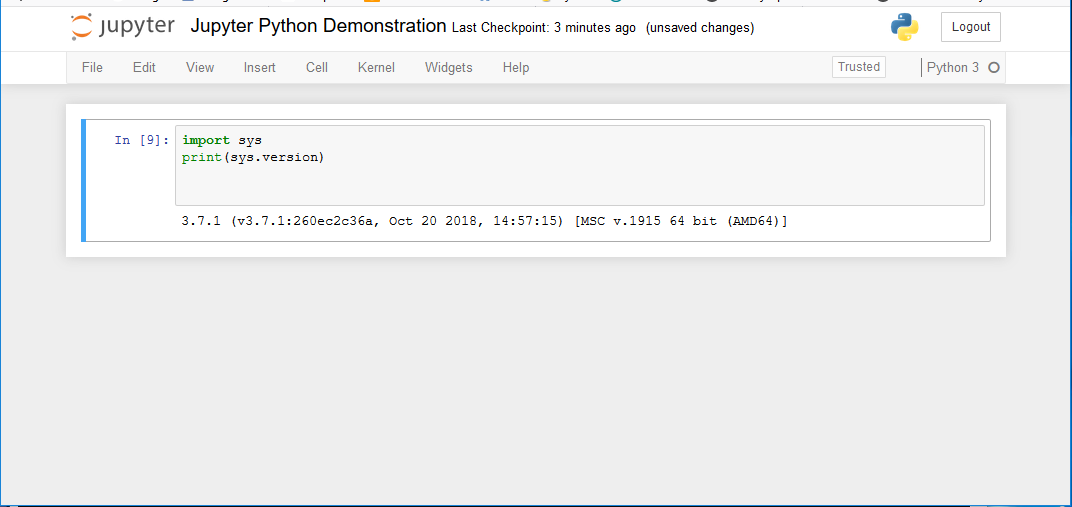
\includegraphics{images/JupyterPythonSession.png}
\caption{Jupyter Python Demo}
\end{figure}

\subsection{Working in rmarkdown and Using R and Python Code
Chunks}\label{working-in-rmarkdown-and-using-r-and-python-code-chunks}

Now consider an index\{rmarkdown\} session running primarily in R. The T
code chunks are executed in the same R session as the rMarkdown. On the
otherhand, a python code chunk is running in a python guest environment
in the R level host using reticulate \index{reticulate}.

Caution: I have found behavior is unpredictible to call R objects back
with Python chunks run in rmarkdown (ie. inside another instance of R).
The identity of R\_User for rpy2 gets lost. There are limits to how
deeply you should nest languages within languages.

That said, the rmarkdown chunks look like this.

\begin{verbatim}
'''{r}
cat("PI in R is", pi)
'''
\end{verbatim}

\begin{verbatim}
'''{python}
import math
print(math.pi)
'''
\end{verbatim}

\chapter{Basic Mathematics in R and
Python}\label{basic-mathematics-in-r-and-python}

This is pretty straight forward and intuitive stuff. Just the same, for
completeness here it is. The Standard libraries of python have the
function beyond the four arithmetic operations.

\section{Add, Subtract, Multiply and
Divide}\label{add-subtract-multiply-and-divide}

\index{syntax} The usual quick calculation would be done in immediate or
interactive mode without relying on print statements. There is outwardly
no difference if the print is used as would be the case in a script.
However Printing a set of values reqires the set be organized into an
object in itself, a vector.

\begin{Shaded}
\begin{Highlighting}[]
\CommentTok{# Loading reticulate package to bring python interpreter on line.}
\KeywordTok{library}\NormalTok{(}\StringTok{"reticulate"}\NormalTok{)}
\end{Highlighting}
\end{Shaded}

\subsection{R Scripting}\label{r-scripting}

\begin{Shaded}
\begin{Highlighting}[]
\CommentTok{# Some immediate calculations, ie. using R like a calculator}
\DecValTok{2} \OperatorTok{+}\StringTok{ }\DecValTok{3}           \CommentTok{# (simple interactive) addition}
\end{Highlighting}
\end{Shaded}

\begin{verbatim}
## [1] 5
\end{verbatim}

\begin{Shaded}
\begin{Highlighting}[]
\DecValTok{5} \OperatorTok{-}\StringTok{ }\DecValTok{2}           \CommentTok{# subtraction}
\end{Highlighting}
\end{Shaded}

\begin{verbatim}
## [1] 3
\end{verbatim}

\begin{Shaded}
\begin{Highlighting}[]
\DecValTok{6} \OperatorTok{*}\StringTok{ }\DecValTok{2}           \CommentTok{# multiplication}
\end{Highlighting}
\end{Shaded}

\begin{verbatim}
## [1] 12
\end{verbatim}

\begin{Shaded}
\begin{Highlighting}[]
\DecValTok{4} \OperatorTok{/}\StringTok{ }\DecValTok{3}           \CommentTok{# division}
\end{Highlighting}
\end{Shaded}

\begin{verbatim}
## [1] 1.333333
\end{verbatim}

\begin{Shaded}
\begin{Highlighting}[]
\KeywordTok{print}\NormalTok{(}\DecValTok{4} \OperatorTok{/}\StringTok{ }\DecValTok{3}\NormalTok{)    }\CommentTok{# calculation in a script requires print to display an answer}
\end{Highlighting}
\end{Shaded}

\begin{verbatim}
## [1] 1.333333
\end{verbatim}

\begin{Shaded}
\begin{Highlighting}[]
\CommentTok{# Variable assignment and printing grouped variables as a vector}
\NormalTok{a <-}\StringTok{ }\NormalTok{(}\DecValTok{2} \OperatorTok{+}\StringTok{ }\DecValTok{3}\NormalTok{)           }\CommentTok{# addition}
\NormalTok{b <-}\StringTok{ }\NormalTok{(}\DecValTok{5} \OperatorTok{-}\StringTok{ }\DecValTok{2}\NormalTok{)           }\CommentTok{# subtraction}
\NormalTok{c <-}\StringTok{ }\NormalTok{(}\DecValTok{6} \OperatorTok{*}\StringTok{ }\DecValTok{2}\NormalTok{)           }\CommentTok{# multiplication}
\NormalTok{d <-}\StringTok{ }\NormalTok{(}\DecValTok{4} \OperatorTok{/}\StringTok{ }\DecValTok{3}\NormalTok{)           }\CommentTok{# division}
\KeywordTok{print}\NormalTok{ (}\KeywordTok{c}\NormalTok{(a, b, c, d))  }\CommentTok{# printing all results together one statement}
\end{Highlighting}
\end{Shaded}

\begin{verbatim}
## [1]  5.000000  3.000000 12.000000  1.333333
\end{verbatim}

Python, on the otherhand considers literal expressions and variables
individually (though we'll see they can be groups as well.) This thr
puthon print statement is by default printing one or more individual
objects as scalars whereas R print function prints object and there is
no scalar. The simplest object in R is the vector.

\subsection{Python Scripting}\label{python-scripting}

The simplest object in python is the scalar, having one of five
\textbf{basic datatypes},

\begin{itemize}
\tightlist
\item
  Integers
\item
  Floating-Point Numbers
\item
  Complex Numbers
\item
  Strings
\item
  Boolean Type
\end{itemize}

\begin{Shaded}
\begin{Highlighting}[]
\CommentTok{# The same immediate calculations, ie. using iPython like a calculator}
\BuiltInTok{print}\NormalTok{(}\DecValTok{2} \OperatorTok{+} \DecValTok{5}\NormalTok{, }\DecValTok{3} \OperatorTok{*} \DecValTok{8}\NormalTok{, }\DecValTok{5} \OperatorTok{-} \DecValTok{1}\NormalTok{, }\DecValTok{67} \OperatorTok{/} \DecValTok{3}\NormalTok{) }\CommentTok{# printing all immediate results together, one statement}
\end{Highlighting}
\end{Shaded}

\begin{verbatim}
## 7 24 4 22.333333333333332
\end{verbatim}

\begin{Shaded}
\begin{Highlighting}[]
\CommentTok{# OR assignment and print}
\NormalTok{a }\OperatorTok{=} \DecValTok{2} \OperatorTok{+} \DecValTok{5}           \CommentTok{# assigned addition}
\NormalTok{b }\OperatorTok{=} \DecValTok{5} \OperatorTok{-} \DecValTok{1}           \CommentTok{# assigned subtraction}
\NormalTok{c }\OperatorTok{=} \DecValTok{3} \OperatorTok{*} \DecValTok{8}           \CommentTok{# assigned multiplication}
\NormalTok{d }\OperatorTok{=} \DecValTok{67} \OperatorTok{/} \DecValTok{3}          \CommentTok{# assigned division}
\BuiltInTok{print}\NormalTok{(a,b,c,d)      }\CommentTok{# printing all results together one statement}
\end{Highlighting}
\end{Shaded}

\begin{verbatim}
## 7 4 24 22.333333333333332
\end{verbatim}

\begin{Shaded}
\begin{Highlighting}[]
\BuiltInTok{print}\NormalTok{(}\StringTok{'a ='}\NormalTok{, a, }\StringTok{'b ='}\NormalTok{,b, }\StringTok{'c ='}\NormalTok{,c, }\StringTok{'d ='}\NormalTok{,d) }\CommentTok{# annotating print is just using 4 literals and 4 variables}
\end{Highlighting}
\end{Shaded}

\begin{verbatim}
## a = 7 b = 4 c = 24 d = 22.333333333333332
\end{verbatim}

This differs from R where a single object is printed but that object may
be a group of objects combined.

\section{Other basic algebraic operators in R and
Python}\label{other-basic-algebraic-operators-in-r-and-python}

\index{syntax} Next lets compare modulus, powers and interger division
in R and python,

\begin{Shaded}
\begin{Highlighting}[]
\DecValTok{35} \OperatorTok\StringTok{ }\DecValTok{2}     \CommentTok{# modulo operator}
\end{Highlighting}
\end{Shaded}

\begin{verbatim}
## [1] 1
\end{verbatim}

\begin{Shaded}
\begin{Highlighting}[]
\DecValTok{35} \OperatorTok\StringTok{ }\DecValTok{2}    \CommentTok{# integer division}
\end{Highlighting}
\end{Shaded}

\begin{verbatim}
## [1] 17
\end{verbatim}

\begin{Shaded}
\begin{Highlighting}[]
\DecValTok{35}\OperatorTok{^}\DecValTok{2}        \CommentTok{# powers in R}
\end{Highlighting}
\end{Shaded}

\begin{verbatim}
## [1] 1225
\end{verbatim}

\begin{Shaded}
\begin{Highlighting}[]
\BuiltInTok{print}\NormalTok{(}\DecValTok{35}\OperatorTok{%}\DecValTok{2}\NormalTok{)       }\CommentTok{# modulo operator}
\end{Highlighting}
\end{Shaded}

\begin{verbatim}
## 1
\end{verbatim}

\begin{Shaded}
\begin{Highlighting}[]
\BuiltInTok{print}\NormalTok{(}\DecValTok{35} \OperatorTok{//} \DecValTok{2}\NormalTok{)    }\CommentTok{# integer division       * note difference from R}
\end{Highlighting}
\end{Shaded}

\begin{verbatim}
## 17
\end{verbatim}

\begin{Shaded}
\begin{Highlighting}[]
\BuiltInTok{print}\NormalTok{(}\DecValTok{35}\OperatorTok{**}\DecValTok{2}\NormalTok{)      }\CommentTok{# powers in python     * note difference from R}
\end{Highlighting}
\end{Shaded}

\begin{verbatim}
## 1225
\end{verbatim}

Note here with python the print statements are required otherwise only
the last immediate calculation would get output to text.

When we extend our algebraic calculations in R the usual functions of
square root, absolute value and exponentiation we still haven't had to
load any library packages. All these are part of the core R.

\begin{Shaded}
\begin{Highlighting}[]
\KeywordTok{abs}\NormalTok{(}\OperatorTok{-}\DecValTok{5}\NormalTok{)          }\CommentTok{# absolute value}
\end{Highlighting}
\end{Shaded}

\begin{verbatim}
## [1] 5
\end{verbatim}

\begin{Shaded}
\begin{Highlighting}[]
\KeywordTok{sqrt}\NormalTok{(}\DecValTok{16}\NormalTok{)         }\CommentTok{# square root function}
\end{Highlighting}
\end{Shaded}

\begin{verbatim}
## [1] 4
\end{verbatim}

\begin{Shaded}
\begin{Highlighting}[]
\KeywordTok{exp}\NormalTok{(}\DecValTok{0}\NormalTok{)           }\CommentTok{# exponent (e^0 etc)}
\end{Highlighting}
\end{Shaded}

\begin{verbatim}
## [1] 1
\end{verbatim}

Not necessarily so for python. We still have the basic functions for
algebraic tasks but from sqrt on ward, we now need to go to the standard
math library for these. As an aside we could have got more powerful
versions of these functions (and more) importing numpy \index{numpy} or
Numba \index{numba} or Scipy \index{Scipy} library packages. This will
come up in more detail later.

\begin{Shaded}
\begin{Highlighting}[]
\BuiltInTok{print}\NormalTok{(}\BuiltInTok{abs}\NormalTok{(}\OperatorTok{-}\DecValTok{5}\NormalTok{))}
\end{Highlighting}
\end{Shaded}

\begin{verbatim}
## 5
\end{verbatim}

\begin{Shaded}
\begin{Highlighting}[]
\BuiltInTok{print}\NormalTok{(}\BuiltInTok{divmod}\NormalTok{(}\DecValTok{10}\NormalTok{,}\DecValTok{3}\NormalTok{))             }\CommentTok{# Returns quotient and remainder of integer division}
\end{Highlighting}
\end{Shaded}

\begin{verbatim}
## (3, 1)
\end{verbatim}

\begin{Shaded}
\begin{Highlighting}[]
\BuiltInTok{print}\NormalTok{(}\BuiltInTok{max}\NormalTok{(}\DecValTok{2}\NormalTok{,}\DecValTok{10}\NormalTok{,}\DecValTok{3}\NormalTok{,}\DecValTok{14}\NormalTok{,}\DecValTok{4}\NormalTok{,}\DecValTok{28}\NormalTok{,}\DecValTok{7}\NormalTok{))    }\CommentTok{# Returns the largest of given arguments or items in an iterable}
\end{Highlighting}
\end{Shaded}

\begin{verbatim}
## 28
\end{verbatim}

\begin{Shaded}
\begin{Highlighting}[]
\BuiltInTok{print}\NormalTok{(}\BuiltInTok{min}\NormalTok{(}\DecValTok{9}\NormalTok{,}\DecValTok{2}\NormalTok{,}\DecValTok{10}\NormalTok{,}\DecValTok{3}\NormalTok{,}\DecValTok{14}\NormalTok{,}\DecValTok{4}\NormalTok{,}\DecValTok{28}\NormalTok{,}\DecValTok{7}\NormalTok{))  }\CommentTok{# Returns the smallest of the given arguments or items in an) iterable}
\end{Highlighting}
\end{Shaded}

\begin{verbatim}
## 2
\end{verbatim}

\begin{Shaded}
\begin{Highlighting}[]
\BuiltInTok{print}\NormalTok{(}\BuiltInTok{pow}\NormalTok{(}\DecValTok{3}\NormalTok{,}\DecValTok{4}\NormalTok{))                   }\CommentTok{# Raises a number to a power}
\end{Highlighting}
\end{Shaded}

\begin{verbatim}
## 81
\end{verbatim}

\begin{Shaded}
\begin{Highlighting}[]
\BuiltInTok{print}\NormalTok{(}\BuiltInTok{round}\NormalTok{(}\FloatTok{3.1415962}\NormalTok{,}\DecValTok{3}\NormalTok{))         }\CommentTok{# Rounds a floating-point value}
\end{Highlighting}
\end{Shaded}

\begin{verbatim}
## 3.142
\end{verbatim}

\begin{Shaded}
\begin{Highlighting}[]
\BuiltInTok{print}\NormalTok{(}\BuiltInTok{sum}\NormalTok{([}\DecValTok{2}\NormalTok{,}\DecValTok{3}\NormalTok{,}\DecValTok{4}\NormalTok{,}\DecValTok{5}\NormalTok{,}\DecValTok{6}\NormalTok{]))       }
\end{Highlighting}
\end{Shaded}

\begin{verbatim}
## 20
\end{verbatim}

\begin{Shaded}
\begin{Highlighting}[]
\ImportTok{import}\NormalTok{ math                     }\CommentTok{# Import \textbackslash{}index\{math package\}/module from \textbackslash{}index\{Standard Library\}}
\BuiltInTok{print}\NormalTok{(math.sqrt(}\DecValTok{16}\NormalTok{))            }\CommentTok{# square root function}
\end{Highlighting}
\end{Shaded}

\begin{verbatim}
## 4.0
\end{verbatim}

\begin{Shaded}
\begin{Highlighting}[]
\BuiltInTok{print}\NormalTok{(math.exp(}\DecValTok{0}\NormalTok{))              }\CommentTok{# exponentiation function (powers of e)}
\end{Highlighting}
\end{Shaded}

\begin{verbatim}
## 1.0
\end{verbatim}

\begin{Shaded}
\begin{Highlighting}[]
\BuiltInTok{print}\NormalTok{(math.log10(}\DecValTok{5}\NormalTok{))            }\CommentTok{# base 10 logarithm}
\end{Highlighting}
\end{Shaded}

\begin{verbatim}
## 0.6989700043360189
\end{verbatim}

\begin{Shaded}
\begin{Highlighting}[]
\BuiltInTok{print}\NormalTok{(math.log(}\DecValTok{5}\NormalTok{))              }\CommentTok{# natural logarithm}
\end{Highlighting}
\end{Shaded}

\begin{verbatim}
## 1.6094379124341003
\end{verbatim}

I suggest, choosing your favorite R introduction and work through it's
early examples using both R and Python - a good chance to try out
Jupyter SOS kernel \index{SOS kernel}. It will also create a record of
the basics of R and python side-by-side that you can refer back to.

A full list of the built-in (as opposed to Standard Library Funtions) is
displayed, from the python documentation, below.

\subsubsection{\texorpdfstring{\href{https://docs.python.org/3.6/library/functions.html}{Python
Built-in
Functions}}{Python Built-in Functions}}\label{python-built-in-functions}

\begin{longtable}[]{@{}lllll@{}}
\toprule
abs() & dict() & help() & min() & setattr()\tabularnewline
all() & dir() & hex() & next() & slice()\tabularnewline
any() & divmod() & id() & object() & sorted()\tabularnewline
ascii() & enumerate() & input() & oct() & staticmethod()\tabularnewline
bin() & eval() & int() & open() & str()\tabularnewline
bool() & exec() & isinstance() & ord() & sum()\tabularnewline
bytearray() & filter() & issubclass() & pow() & super()\tabularnewline
bytes() & float() & iter() & print() & tuple()\tabularnewline
callable() & format() & len() & property() & type()\tabularnewline
chr() & frozenset() & list() & range() & vars()\tabularnewline
classmethod() & getattr() & locals() & repr() & zip()\tabularnewline
compile() & globals() & map() & reversed() &
\textbf{import}()\tabularnewline
complex() & hasattr() & max() & round() &\tabularnewline
delattr() & hash() & memoryview() & set() &\tabularnewline
\bottomrule
\end{longtable}

R has a very large set of built-in functions available before the need
to load any libraries arises. The
\href{https://cran.r-project.org/doc/manuals/r-release/R-lang.html}{R
Language Reference} provides a comprehensive background on built in
fucntions as well as the rest of the language.

So R is centered around the mandate of being a complete mathematical
system, much like Matlab,(Octave or SciLab) which Python's mandate is
that of a full featured scripting and programming environment.

However, calling \index{standard library} modules in python puts it
quite easily and effectively on a even par with R. Going into more
complex activites requires thar both load or import fucther libraries.
Like
\href{https://docs.python.org/3/library/index.html}{\textbf{Python's
Standard Library}}, \textbf{the R Core Library} shipping with the R
install is described in the
\href{https://cran.r-project.org/doc/manuals/r-release/fullrefman.pdf}{Full
R Reference Manual} and covers a wide range of mathematical, statistical
and programming solutions.

We will go deeper into these and the other external Libraries and
modules in the next chapter, covering functional programming in more
detail. As well focused discussions on specific Data Science domains
form a block of Chapters in Part II of the book.

\chapter{Functional Programming with R and
Python}\label{functional-programming-with-r-and-python}

At this point we are ready to discuss the functional programming
paradigm in R and Python. The other important paradigm, Object-Oriented,
will be discussed in the following Chapter.

In using python in a functional paradigm, a script is built as a series
of functions. Data is passed through one of more functions (ie. as
series of functions) to carry out steps of a larger task set. When data
is passed to a function to carry out some task or analysis on a dataset
results may then printed out directly, stored in memory or on disk, or
displayed in graphical form by passing the analysis to another set of
functions such as those of matplotlib \index{matplotlib} for plotting
etc.

A function is a set of stored programmatic statements stored in an
accessible form for reuse. The function is called in R or Python by
simply inserting it by name in a statement to be executed by one of the
interpreters.

\section{Defining Functions}\label{defining-functions}

A function is defined in a specific format for each language.

\subsection{R Scripting}\label{r-scripting-1}

\begin{Shaded}
\begin{Highlighting}[]
\NormalTok{doArea <-}\StringTok{ }\ControlFlowTok{function}\NormalTok{(radius)\{}
\NormalTok{  area <-}\StringTok{ }\NormalTok{pi }\OperatorTok{*}\StringTok{ }\NormalTok{radius}\OperatorTok{^}\DecValTok{2}
\NormalTok{\}}
\end{Highlighting}
\end{Shaded}

\subsection{Python Scripting}\label{python-scripting-1}

\begin{Shaded}
\begin{Highlighting}[]
\ImportTok{import}\NormalTok{ math}
\KeywordTok{def}\NormalTok{ calcArea(radius):}
\NormalTok{  area }\OperatorTok{=}\NormalTok{ math.pi }\OperatorTok{*}\NormalTok{ radius}\OperatorTok{**}\DecValTok{2}
  \ControlFlowTok{return}\NormalTok{ area}
\end{Highlighting}
\end{Shaded}

\section{Calling and Using Functions}\label{calling-and-using-functions}

\subsection{R Scripting}\label{r-scripting-2}

\begin{Shaded}
\begin{Highlighting}[]
\NormalTok{radius =}\StringTok{ }\DecValTok{4}
\KeywordTok{print}\NormalTok{(}\KeywordTok{doArea}\NormalTok{(radius))}
\end{Highlighting}
\end{Shaded}

\begin{verbatim}
## [1] 50.26548
\end{verbatim}

\begin{Shaded}
\begin{Highlighting}[]
\NormalTok{x =}\StringTok{ }\KeywordTok{doArea}\NormalTok{(}\DecValTok{4}\NormalTok{) }\OperatorTok{+}\StringTok{ }\DecValTok{100}
\KeywordTok{print}\NormalTok{(x)}
\end{Highlighting}
\end{Shaded}

\begin{verbatim}
## [1] 150.2655
\end{verbatim}

\subsection{Python Scripting}\label{python-scripting-2}

\begin{Shaded}
\begin{Highlighting}[]
\ImportTok{import}\NormalTok{ math}
\KeywordTok{def}\NormalTok{ calcArea(radius):}
\NormalTok{  area }\OperatorTok{=}\NormalTok{ math.pi }\OperatorTok{*}\NormalTok{ radius}\OperatorTok{**}\DecValTok{2}
  \ControlFlowTok{return}\NormalTok{ area}
\BuiltInTok{print}\NormalTok{(calcArea(}\DecValTok{4}\NormalTok{))}
\end{Highlighting}
\end{Shaded}

\begin{verbatim}
## 50.26548245743669
\end{verbatim}

Let's discuss the differences in how the functions were called to be
used. COnsider first that the book is set-up as written in rMarkdown
which is running in an instance of R. The memory of the code chunk and
the underling R which rmarkdown is running are the same. In python
terms, the namespace is the same. This is not the case with the python
code chunks. We have to explicitly pass to (and retrieve from) the R
namespace \index{namespace} for it to be accessible to the python chunk,
running in it's on (python) namespace. As a result we had to redefine
the function in the same namespace in which we were calling it.

With R code chunks the R memory space is open throughout but the python
chunks name space is closed each time the python chunk closes. This is a
feature of how I am using the R environment to write this book, not of
python per se.

Further, recalling we are writing scripts, the print statements are
required for both to display the result. We could have used the cat()
function of course to display the R output as well.

\begin{Shaded}
\begin{Highlighting}[]
\KeywordTok{cat}\NormalTok{(x)       }\CommentTok{# x is still in R memory here}
\end{Highlighting}
\end{Shaded}

\begin{verbatim}
## 150.2655
\end{verbatim}

Note that the result number {[}1{]} is not printed with R using cat() or
the python print() functions.

There are more subtlies of memory management in calling one language
from inside the other. These will come up below but for now knowing how
things behave in the R/rMarkdown environment as above will cover our
memory space issues.

\section{Writing Function Examples in R and
Python}\label{writing-function-examples-in-r-and-python}

\subsubsection{Example 1 A Surveyor's
Function}\label{example-1-a-surveyors-function}

Lets write a function in R and Python to calculate the height of a tower
knowing the angle of elevation at a given distance from the base. This
would be something we might need when sighting through a surveyors
transit.

Given a distance from the base of 1000 meters, how high is a tower whose
top was measured at an angle of 25 degrees at that distance.

\begin{Shaded}
\begin{Highlighting}[]
\NormalTok{d =}\StringTok{ }\DecValTok{1000}    \CommentTok{# distance in meters to base}
\NormalTok{ad =}\StringTok{ }\DecValTok{25}     \CommentTok{# angle in degrees}

\CommentTok{# write a function to convert degrees to radians}
\NormalTok{deg2rad =}\StringTok{ }\ControlFlowTok{function}\NormalTok{(angledeg)\{}
\NormalTok{  angledeg }\OperatorTok{*}\StringTok{ }\NormalTok{(pi}\OperatorTok{/}\DecValTok{180}\NormalTok{)}
\NormalTok{\}}

\CommentTok{# write function to calcular height from angle in degrees}
\NormalTok{ht =}\StringTok{ }\ControlFlowTok{function}\NormalTok{(d, ad)\{}
\NormalTok{  h =}\StringTok{ }\NormalTok{d}\OperatorTok{*}\KeywordTok{tan}\NormalTok{(}\KeywordTok{deg2rad}\NormalTok{(ad))}
\NormalTok{\}}

\CommentTok{# now call and output function with distance d and angle ad in degrees}
\KeywordTok{cat}\NormalTok{(}\StringTok{"Tower Height in meters is: "}\NormalTok{, }\KeywordTok{ht}\NormalTok{(d, ad), }\StringTok{"}\CharTok{\textbackslash{}n}\StringTok{"}\NormalTok{)    }
\end{Highlighting}
\end{Shaded}

\begin{verbatim}
## Tower Height in meters is:  466.3077
\end{verbatim}

So we have written 2 functions, one to convert degrees to radians, that
is the expected measure of the angle going into ttigonometric functions
of R. Then we wrote a function to accept degrees input and give the
height in meters (the input distance units) The function definitions use
the keyword `function, followed by zero or more arguments and then the
code block of the function is set out by brace brackets'\{ \}'. The
function is assigned to a name like a variable.

Lets do it with python now,

\begin{Shaded}
\begin{Highlighting}[]
\CommentTok{# set variables to problem givens}
\NormalTok{d }\OperatorTok{=} \DecValTok{1000}    \CommentTok{# distance in meters to base}
\NormalTok{ad }\OperatorTok{=} \DecValTok{25}     \CommentTok{# angle in degrees}
\CommentTok{# write a function to convert degrees to radians}
\KeywordTok{def}\NormalTok{ deg2rad(angledeg):}
    \ImportTok{import}\NormalTok{ math}
    \ControlFlowTok{return}\NormalTok{(angledeg }\OperatorTok{*}\NormalTok{ (math.pi}\OperatorTok{/}\DecValTok{180}\NormalTok{))}
    
\CommentTok{# write function to calcular height from angle in degrees}
\KeywordTok{def}\NormalTok{ ht(d, ad):}
  \ImportTok{import}\NormalTok{ math}
  \ControlFlowTok{return}\NormalTok{ (d}\OperatorTok{*}\NormalTok{math.tan(deg2rad(ad)))}
\CommentTok{# now call and output function with distance d and angle ad in degrees}
\BuiltInTok{print}\NormalTok{(}\StringTok{"The height in meters of the tower is :"}\NormalTok{, ht(d, ad))}
\end{Highlighting}
\end{Shaded}

\begin{verbatim}
## The height in meters of the tower is : 466.3076581549986
\end{verbatim}

In the python declarations the definition starts with the keyword `def'
a name and zero or more arguments and there is a colon `:' at the end of
the first line. The code block of the function is also indented rather
than set out by brace brakets `\{ \}'. The first line is the signature
of the function.

Both functions return a value, typically the last value in the
calculation chain for R but as an explicitly called return for python.
Note for the two python functions one has a space after return and the
other doesn't. This is because the bracket do not contain return
parmeters but group the expression to be returned.

Also as previously alluded to pi in R is a core CONSTANT but in python
it is a CONSTANT in the math module which must be imported to use it. We
could have just explicitly imported only pi at the start and referred to
it directly by name as in R.

\begin{verbatim}
# Python code
 print(pi)


Gives an error:

 Traceback (most recent call last):
   File "C:\Users\medma\AppData\Local\Temp\RtmpYlYLtl\chunk-code-148c67392482.txt", line 1, in
   <module>
     print(pi)
 NameError: name 'pi' is not defined
\end{verbatim}

\begin{Shaded}
\begin{Highlighting}[]
\ImportTok{from}\NormalTok{ math }\ImportTok{import}\NormalTok{ pi}
\BuiltInTok{print}\NormalTok{(pi)}
\end{Highlighting}
\end{Shaded}

\begin{verbatim}
## 3.141592653589793
\end{verbatim}

Once again you must know where to go to get some constants and functions
with python which are built-in in R. Check out the math module
\index{math module} in the standard python library\textsuperscript{3}.
\index{standard python library}

\section{Using the Core R and Python Standard
Libraries}\label{using-the-core-r-and-python-standard-libraries}

\index{syntax} Core R distributions currently install with a base set of
function packages. The Table in the
\href{17-Appendix_3_Packages.Rmd}{Appendix 3} lists these.

The python standard libraries contain alot of modules which can be
imported. They are grouped in modules by functionality. The functions
contained in the modules can be looked up in the
\href{https://docs.python.org/3.7/}{Official Documentation} online or
referring to the Hellmann\textsuperscript{2} book.

As done for the R base system in the Appendix, I also list the groups of
python modules of the Standard Library in the Appendix 3 by kind as in
the Python Documentation\textsuperscript{3}, but generally including
only occasional examples of the many functions each contain. Again a
more exhaustive handling is available as indicated.

It's a good time to dive into the functions of the core libraries and
try some more sophisticated R and Python tasks. We'll first compare
loading and saving datasets in both languages. R has file functions for
saving dataframes as comma separated variables, csv, files. We will then
load this data back into R and python to compare these tasks in each.

\subsection{R Scripting}\label{r-scripting-3}

The \index{dataframe} \index{airquality} is a built in dataset. Rather
than display the whole tales head(n) \index{head(n)} displays the first
n lines (default n=6). Similarly tail(n) \index{tail(n)} would display
the last n lines. The named dataframe `table' is created from airquality
data. Then we tell R to write a file names airquality.csv with write.csv
\index{write.csv}. R automatically closes the file after writing is
complete.

\begin{Shaded}
\begin{Highlighting}[]
\CommentTok{# loading dataset from base R called }
\KeywordTok{head}\NormalTok{(airquality)}
\end{Highlighting}
\end{Shaded}

\begin{verbatim}
##   Ozone Solar.R Wind Temp Month Day
## 1    41     190  7.4   67     5   1
## 2    36     118  8.0   72     5   2
## 3    12     149 12.6   74     5   3
## 4    18     313 11.5   62     5   4
## 5    NA      NA 14.3   56     5   5
## 6    28      NA 14.9   66     5   6
\end{verbatim}

\begin{Shaded}
\begin{Highlighting}[]
\NormalTok{table =}\StringTok{ }\NormalTok{airquality}
\KeywordTok{write.csv}\NormalTok{(table,}\DataTypeTok{file=}\StringTok{"airquality.csv"}\NormalTok{)}
\end{Highlighting}
\end{Shaded}

\subsection{Python Scripting}\label{python-scripting-3}

We need the io module for the file access function. The open() function
opens the file ``airquality.csv'' for reading only (``r'') and creates a
filehandle, we called file. Now, file is a handle object so here is a
first nod to OOP dotted function syntax to read a line from it.
Something more functionally intuitive, like \texttt{readline(file)} will
yield an error. Because calling of R function use dot syntax calls this
is not new to us here. Next chapter moves fully to OOP paradigm.

Then we print out what we read - a single line from file (in fact, the
first line)

\begin{Shaded}
\begin{Highlighting}[]
\CommentTok{# Needs io module functions}
\ImportTok{import}\NormalTok{ io}
\CommentTok{#load csv data with Python }
\BuiltInTok{file} \OperatorTok{=} \BuiltInTok{open}\NormalTok{(}\StringTok{"airquality.csv"}\NormalTok{, }\StringTok{"r"}\NormalTok{)}
\NormalTok{aline }\OperatorTok{=} \BuiltInTok{file}\NormalTok{.readline()}
\BuiltInTok{print}\NormalTok{(aline)}
\end{Highlighting}
\end{Shaded}

\begin{verbatim}
## "","Ozone","Solar.R","Wind","Temp","Month","Day"
\end{verbatim}

\begin{Shaded}
\begin{Highlighting}[]
\NormalTok{aline }\OperatorTok{=} \BuiltInTok{file}\NormalTok{.readline()}
\BuiltInTok{print}\NormalTok{(aline)}
\end{Highlighting}
\end{Shaded}

\begin{verbatim}
## "1",41,190,7.4,67,5,1
\end{verbatim}

\begin{Shaded}
\begin{Highlighting}[]
\BuiltInTok{file}\NormalTok{.close}
\end{Highlighting}
\end{Shaded}

When we read a line again, we read the next line. Python readline
maintains a pointer it moves as we continue to readlines. The Two lines
we printer were the column names as we saved them and a line of comma
separated values.

Lets read the airquality.csv file back into R assigning a name
``newtable'' to the dataframe the read.csv \index{read.csv} command
creates to store the data loaded.

\begin{Shaded}
\begin{Highlighting}[]
\CommentTok{# Load csv data with R}
\NormalTok{newtab =}\StringTok{ }\KeywordTok{read.csv}\NormalTok{(}\DataTypeTok{file=}\StringTok{"airquality.csv"}\NormalTok{, }\DataTypeTok{header=}\OtherTok{TRUE}\NormalTok{)}
\KeywordTok{head}\NormalTok{(newtab)}
\end{Highlighting}
\end{Shaded}

\begin{verbatim}
##   X Ozone Solar.R Wind Temp Month Day
## 1 1    41     190  7.4   67     5   1
## 2 2    36     118  8.0   72     5   2
## 3 3    12     149 12.6   74     5   3
## 4 4    18     313 11.5   62     5   4
## 5 5    NA      NA 14.3   56     5   5
## 6 6    28      NA 14.9   66     5   6
\end{verbatim}

R automatically loads the csv data back into a dataframe. However, the
python readline reads the data as a data stream (a stream of characters)
which we told it to store in the aline variable. python does not in this
case parse the stream int any special structure - that is left to us to
do.

We see something else too. R wrote the row numbers to the file (because
we didn't say otherwise) and assigned a new set again when we loaded the
data again.

\subsection{More Function Examples}\label{more-function-examples}

Basic plotting functions are part of the r-base system we can easily
plot a function, \index{syntax}

\begin{Shaded}
\begin{Highlighting}[]
\CommentTok{# Create a function to make a line plot or squares of x between 1 and 8}
\NormalTok{linePlotMySquares <-}\ControlFlowTok{function}\NormalTok{(}\DataTypeTok{type =} \StringTok{"l"}\NormalTok{, ...) \{}
\NormalTok{  x =}\StringTok{ }\KeywordTok{c}\NormalTok{(}\DecValTok{1}\NormalTok{,}\DecValTok{2}\NormalTok{,}\DecValTok{3}\NormalTok{,}\DecValTok{4}\NormalTok{,}\DecValTok{5}\NormalTok{,}\DecValTok{6}\NormalTok{,}\DecValTok{7}\NormalTok{,}\DecValTok{8}\NormalTok{)}
\NormalTok{  y =}\StringTok{ }\NormalTok{x}\OperatorTok{**}\DecValTok{2}
  \KeywordTok{plot}\NormalTok{(x, y, }\DataTypeTok{type =}\NormalTok{ type, ...)}
\NormalTok{\}}

\CommentTok{# Call our function}
\KeywordTok{linePlotMySquares}\NormalTok{()}
\end{Highlighting}
\end{Shaded}

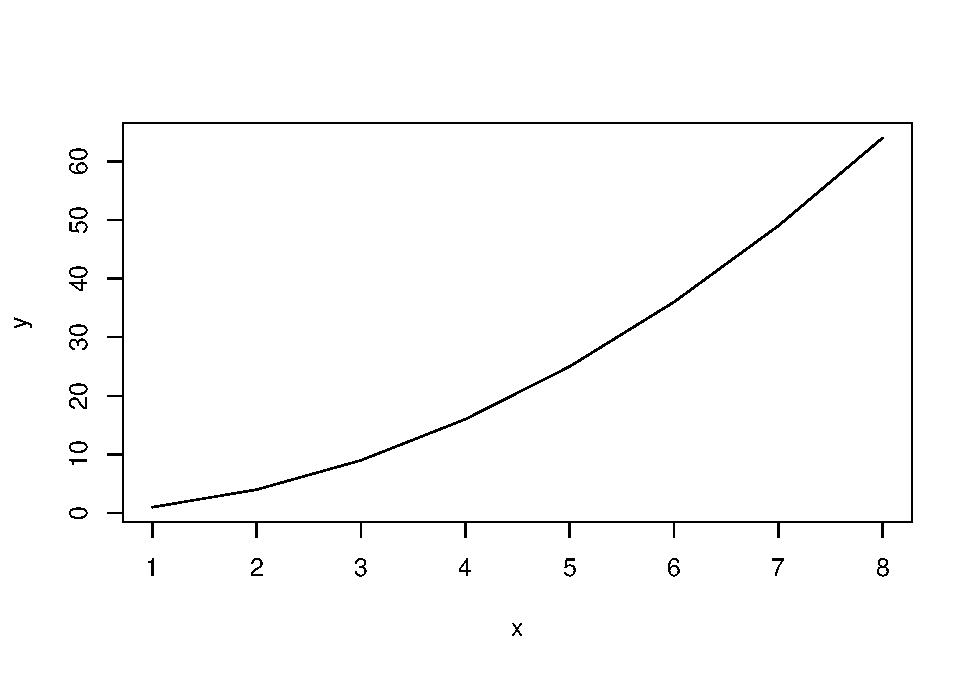
\includegraphics{RPythonBook_files/figure-latex/unnamed-chunk-26-1.pdf}

Python does not have a basic plotting function and the Standard Library
has not provided one either. You casn write your own but there is a
popular python library from the Scipy \index{Scipy} folks called
Matplotlib which once installed from the shell with PIP \index{PIP},

\begin{verbatim}
> pip install matplotlib

OR

> python -m pip install matplotlib
\end{verbatim}

is available for import, and it contains a module called pyplot which
has a simple plot function

\index{syntax}

\begin{Shaded}
\begin{Highlighting}[]
\ImportTok{from}\NormalTok{ matplotlib }\ImportTok{import}\NormalTok{ pyplot }\ImportTok{as}\NormalTok{ plt  }\CommentTok{# import pyplot library module from matplotlib}
\NormalTok{x }\OperatorTok{=} \BuiltInTok{list}\NormalTok{(}\BuiltInTok{range}\NormalTok{(}\DecValTok{1}\NormalTok{,}\DecValTok{11}\NormalTok{))                  }\CommentTok{# make a sequence of numbers from 1 through 8, called x}
\NormalTok{y }\OperatorTok{=}\NormalTok{ [}\DecValTok{0}\NormalTok{,]                              }\CommentTok{# create a list, must have at least one element to concat to}
\ControlFlowTok{for}\NormalTok{ val }\KeywordTok{in}\NormalTok{ x:                         }\CommentTok{# loop through list x to calculate squares}
\NormalTok{    y }\OperatorTok{=}\NormalTok{ y }\OperatorTok{+}\NormalTok{ [val}\OperatorTok{**}\DecValTok{2}\NormalTok{,]                 }\CommentTok{# concatinate each square to list y as calculated}
\NormalTok{y }\OperatorTok{=}\NormalTok{ y[}\DecValTok{1}\NormalTok{:}\DecValTok{11}\NormalTok{]                            }\CommentTok{# select the values 1 to 8 from y, call them y}
\NormalTok{plt.plot(x,y)                         }\CommentTok{# plot the x vs y pairs}
\NormalTok{plt.show()                            }\CommentTok{# show the plot}
\end{Highlighting}
\end{Shaded}

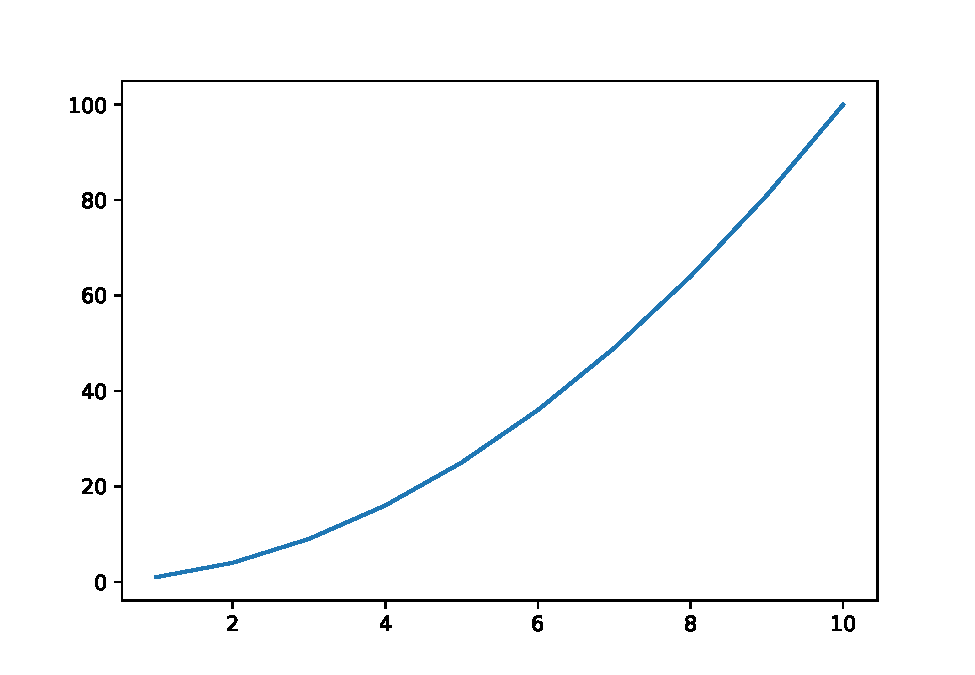
\includegraphics{RPythonBook_files/figure-latex/unnamed-chunk-27-1.pdf}

There are a few things to discuss here. First is the structure of the
matplotlib library. Python code for import are module files (which end
in the .py extension like any python scripts or programs).

\begin{quote}
A script or program is generally a directly executable piece of code,
run by itself. A module is generally a library, imported by other pieces
of code.
\end{quote}

\begin{quote}
Note that there's no internal distinction -- both are executable and
importable, although library code often won't do anything (or will just
run its unit tests) when executed directly and importing code designed
to be a script will cause it to execute, hence the common if
\textbf{name} == ``\textbf{main}'' test.\textsuperscript{17}
\end{quote}

So what we are doing with
\texttt{from\ matplotlib\ import\ pyplot\ as\ plt} is saying: ``from the
file matploylib \index{matplotlib}(.py) \index{pyplot} import the
functions in the pyplot class and call the namespace containing them
plt'' \index{namespace}so that we can call them.

\textbf{Note:} PIP \index{PIP} is a module, but runs independently from
the command line because it contains script with a \texttt{\_\_main\_\_}
function accessed via pip3.exe to setup and start the process.

It also runs from command line as a module executed by python with the
-m switch, by

\begin{verbatim}
python -m pip install <some package>
\end{verbatim}

the -m switch \index{-m switch} tells python to run the module as a
script. Most library modules are not executable as python scripts or if
they are, run self-tests called by a main() function.

\chapter{Object-Oriented Programming with R and
Python}\label{object-oriented-programming-with-r-and-python}

At this point we are ready to expand our exploration with
object-oriented programming (OOP) in R and Python. Objects are like
(collections of one or more) functions with some added structure. This
structure has been defined by the four principles which set apart OOP.

\begin{itemize}
\tightlist
\item
  Abstarction \index{Abstraction}.
\item
  Encapsulation \index{Encapsulation}.
\item
  Inheritance \index{Inheritance}.
\item
  Polymorphism \index{Polymorphism}.
\end{itemize}

Additionally the functions an object contains, called it's methods are
conceptualized as relating to the actions of the object. The methods are
actions which are done by the object for itself - an add method enables
the object to add itself. A square object would add something to itself
in an internally defined fashion.

Consider a function/method to transparently operates on a variable as
would be appropriate to the data-type. This is \textbf{polymorphism}, a
consequence of the message-passing \index{message-passing} model. An
`add' method would do some sort of add operation in a fashion
appropriate to the object and the input, and it would do it by passing a
``do add''" message into the blackbox of the object and the details are
inaccessible to the user. Access to the objects characteristics is also
by such methods and in no other way. This is \textbf{encapsulation} or
`information hiding'.

You can only alter an object itself by extending it's pattern in a new
object. All the things of the old object are passed on and exist in the
new object by re-inplementation of old characteristics and new
characteristics and behaviors are implemented on top of the parent
object's pattern. This is \textbf{inheritance}.

As above the object has control over how it is seen in the environment
external to the object. The picture the object releases is an
\textbf{abstraction} of it's pattern definition and contents. The
totality of object data structure emerges from the outputs of the object
methods.

A generic class pattern\index{class pattern} or definition (in
pseudocode) consists of a class signature (or name) and a contained code
block with class details. This is the fundamental abstraction which is
an object. It could be represented like this,

\begin{verbatim}
# Class indentity
class() [ include inheritance]

    #Class details
    # the characteristics
    class constants 
    class variables
  
    # instance creation
    constructor()
    
    # class actions
    methods()
\end{verbatim}

\section{Defining Classes in R and
Python}\label{defining-classes-in-r-and-python}

A class is a specific object pattern, The automobile class is an object
with wheels, some mode of propulsion and driver methods. A class
instance is a particular realization of car with specifics values added
to characteristics inherited from the class.

\textbf{R, Functions or Classes}

Due to how it evolved, R has at least 3 kinds or levels of objects,
developed in a chronologic order. These all, arguably, then strain the
limits of what is or is not Object-Oriented. The explanation
offered\textsuperscript{22} is the origin of R from S as an interactive
environment and further development faces compromises to this. It can be
used as a scripting language, even as if running programs but at the
base of it all the interpreter runs the scripts in the the main over
it's interactive nature.

I think in an important sense none of the OOP attempts fit the bill.
Witness that there are 3 attempts to provide an R environment for
Object-Oriented development and all have different shortcomings in the
implementation. Add further what is actually a 4th object-oriented-type,
but outside of core-R, with the \href{https://github.com/r-lib/R6/}{R6
Package}. Summarizing,

\begin{itemize}
\tightlist
\item
  \index{S3} (predominantly genertic functions without formal class
  definition)
\item
  \index{S4} (Class definitions)
\item
  RC (\index{Reference Class}es, or `euphemistically' S5 or \index{R5})
\item
  \index{R6} (External to Core-R R6 package)
\end{itemize}

The result of all this is that only the masochistically R obscessed or
extreme programmer ventures here. R scripting afficionados even with
lots of time proceed with caution.

I learned Object-Oriented Programming with Java and statistics with R.
After a look further inside R for OOP, I decided I wasn't going there -
all the more reason for adding Python to one's Data Science repertoir.

I am not going to explore R OOP \index{R OOP} beyond the discussion
under calling R objects below, really \emph{a syntatic variant} of
functional programming. Those readers truly coming from R will
understand. \index{syntax}

\textbf{Python Objects}

In contrast to R python Object-Oriented Programming meets nearly
everybody's understanding of OOP. Python Objects \index{Python Objects}
when instantiated look, feel and behave like an object for me. The
python system of namespaces \index{namespace}s and variable visability
blend consistently with the idea of encapsulation and data-hiding.

Python objects inherit from parent objects as expected and polymorphism
operates behind the object envelope transparently and as one logicall
expects for data-types or structures. Abstraction is a conceptualization
of the data-structres created as objects.

Lets create a simple python class\textsuperscript{8-p627} like,
\index{syntax}

\begin{Shaded}
\begin{Highlighting}[]
\CommentTok{# python code}
\KeywordTok{class}\NormalTok{ SimpleClass:                 }
  \CommentTok{# Define the class object}
  
  \CommentTok{# Note: Implied constructor is  }
  \CommentTok{#    that of the base object of  }
  \CommentTok{#    the python environment.}
  
  \CommentTok{# Define class methods}
  \KeywordTok{def}\NormalTok{ setdata(}\VariableTok{self}\NormalTok{, value):       }\CommentTok{# a value 'setter' method}
    \VariableTok{self}\NormalTok{.value }\OperatorTok{=}\NormalTok{ value            }\CommentTok{#   \textbackslash{}index\{self\} is the instance itself}
  \KeywordTok{def}\NormalTok{ getdata(}\VariableTok{self}\NormalTok{):              }\CommentTok{# a value 'getter' method}
    \BuiltInTok{print}\NormalTok{(}\VariableTok{self}\NormalTok{.value)}
    
\CommentTok{# create object instance from class definition}
\NormalTok{x }\OperatorTok{=}\NormalTok{ SimpleClass()}
\NormalTok{x.setdata(}\DecValTok{5}\NormalTok{)                      }\CommentTok{# x became '\textbackslash{}index\{self\}' in the abstract}
\NormalTok{x.getdata()                       }\CommentTok{# what is the value of x}
\end{Highlighting}
\end{Shaded}

\begin{verbatim}
## 5
\end{verbatim}

\begin{Shaded}
\begin{Highlighting}[]
\BuiltInTok{print}\NormalTok{(x.value)}
\end{Highlighting}
\end{Shaded}

\begin{verbatim}
## 5
\end{verbatim}

Well, now we just accessed the value of x directly - not hidden data as
we should expect.

Let's try another, the ubiquitous Car example \index{Car example}.
\index{syntax}

\begin{Shaded}
\begin{Highlighting}[]
\CommentTok{# what is a car?}
\KeywordTok{class}\NormalTok{ Car:}
\NormalTok{  _motor }\OperatorTok{=} \StringTok{""}
\NormalTok{  _style }\OperatorTok{=} \StringTok{""}
\NormalTok{  _year }\OperatorTok{=} \StringTok{""}
  
  \KeywordTok{def} \FunctionTok{__init__}\NormalTok{(}\VariableTok{self}\NormalTok{, year, style, motor):      }\CommentTok{# constructor, always an __init__ function}
    \VariableTok{self}\NormalTok{._motor}\OperatorTok{=}\NormalTok{motor}
    \VariableTok{self}\NormalTok{._style}\OperatorTok{=}\NormalTok{style}
    \VariableTok{self}\NormalTok{._year}\OperatorTok{=}\NormalTok{year}
    
  \KeywordTok{def}\NormalTok{ setmotor(}\VariableTok{self}\NormalTok{, motor):       }\CommentTok{# setters}
    \VariableTok{self}\NormalTok{._motor}\OperatorTok{=}\NormalTok{motor}
    
  \KeywordTok{def}\NormalTok{ setstyle(}\VariableTok{self}\NormalTok{, style):}
    \VariableTok{self}\NormalTok{._style}\OperatorTok{=}\NormalTok{style}
    
  \KeywordTok{def}\NormalTok{ getmotor(}\VariableTok{self}\NormalTok{):              }\CommentTok{# getters}
    \ControlFlowTok{return}\NormalTok{ _self.motor}
    
  \KeywordTok{def}\NormalTok{ getstyle(}\VariableTok{self}\NormalTok{): }
    \ControlFlowTok{return}\NormalTok{ _self.style}
    
  \KeywordTok{def}\NormalTok{ toString(}\VariableTok{self}\NormalTok{):}
    \ControlFlowTok{return}\NormalTok{ (}\VariableTok{self}\NormalTok{._year}\OperatorTok{+}\StringTok{","}\OperatorTok{+}\VariableTok{self}\NormalTok{._motor}\OperatorTok{+}\StringTok{","}\OperatorTok{+}\VariableTok{self}\NormalTok{._style)}
    
    
\CommentTok{# build a car}
\NormalTok{Newcar }\OperatorTok{=}\NormalTok{ Car(}\StringTok{'2019'}\NormalTok{,}\StringTok{'Sedan'}\NormalTok{, }\StringTok{'4 cylinder gasoline'}\NormalTok{ )}
\CommentTok{# What is 'our' Newcar?}
\BuiltInTok{print}\NormalTok{(Newcar)}
\end{Highlighting}
\end{Shaded}

\begin{verbatim}
## <__main__.Car object at 0x0000000064B48CF8>
\end{verbatim}

OOoops I printed out the object info
\index{object info vs instance data} not the instance data!

What happens if I try direct access to an instance variable `style'?

\begin{verbatim}
print(Newcar.style)
\end{verbatim}

We get an error,

\begin{verbatim}
Error in py_run_string_impl(code, local, convert) : 
  AttributeError: 'Car' object has no attribute 'style'

Detailed traceback: 
  File "<string>", line 1, in <module>
Calls: <Anonymous> ... py_capture_output -> force -> py_run_string -> py_run_string_impl
Execution halted
\end{verbatim}

Unfortunately, it is still accessible but you need to use the internal
name '\_style'

\begin{Shaded}
\begin{Highlighting}[]
\BuiltInTok{print}\NormalTok{(Newcar._style)}
\end{Highlighting}
\end{Shaded}

\begin{verbatim}
## Sedan
\end{verbatim}

Well in terms of encapsulation in python OOP, close but no cigar. But as
\href{https://medium.com/@leandrotk_}{leandrotk} notes in
\href{https://medium.com/the-renaissance-developer/python-101-object-oriented-programming-part-2-8e0db3ddd531}{this
blog} \index{Non-public variablesas convention}

\begin{quote}
Non-public variables are just a convention and should be treated as a
non-public part of the API.
\end{quote}

That means when we see the leading underscore \index{leading underscore}
weare `pretending' the variable is private. The responsibility rests
with the programmer. The only way to control it at all is to not
document the underscore for the object's API.

Now try again using the object's own print method.

\begin{Shaded}
\begin{Highlighting}[]
\BuiltInTok{print}\NormalTok{(Newcar.toString())}
\end{Highlighting}
\end{Shaded}

\begin{verbatim}
## 2019,4 cylinder gasoline,Sedan
\end{verbatim}

What about inheritance? Let's subclass the car as a truck.

\begin{Shaded}
\begin{Highlighting}[]
\KeywordTok{class}\NormalTok{ Truck(Car):}
\NormalTok{    _type }\OperatorTok{=} \StringTok{""}
    \KeywordTok{def} \FunctionTok{__init__}\NormalTok{(}\VariableTok{self}\NormalTok{, year, style, motor, }\BuiltInTok{type}\NormalTok{):}
        \BuiltInTok{super}\NormalTok{().}\FunctionTok{__init__}\NormalTok{(year, style, motor)}
        \VariableTok{self}\NormalTok{._type }\OperatorTok{=} \BuiltInTok{type}
   
    \KeywordTok{def}\NormalTok{ toString(}\VariableTok{self}\NormalTok{):}
        \ControlFlowTok{return} \BuiltInTok{super}\NormalTok{().toString() }\OperatorTok{+} \StringTok{","} \OperatorTok{+} \VariableTok{self}\NormalTok{._type}
        
\NormalTok{Bigtruck }\OperatorTok{=}\NormalTok{ Truck(}\StringTok{'2018'}\NormalTok{,}\StringTok{'Truck'}\NormalTok{,}\StringTok{'6 cylinder diesel'}\NormalTok{, }\StringTok{'box'}\NormalTok{ )}
\BuiltInTok{print}\NormalTok{(Bigtruck.toString())}
\end{Highlighting}
\end{Shaded}

\begin{verbatim}
## 2018,6 cylinder diesel,Truck,box
\end{verbatim}

We have used the car pattern, referring to it as the superclass super.
and we have overridden the tostring function to include the \_type
variable appended to the car string.

\section{Using Objects and Classes}\label{using-objects-and-classes}

An instance of a class is created by the class constructor
\index{constructor}. An object constructor is implicitly inherited by
all classes, from the language's object definition and implementation.
It is often explicitly overridden by a customized contructor.

\subsection{R Scripting}\label{r-scripting-4}

\subsection{Python Scripting}\label{python-scripting-4}

\part{Data Science Topics in Python Compared to
R}\label{part-data-science-topics-in-python-compared-to-r}

\chapter{Clean and Tidy Data}\label{clean-and-tidy-data}

\index{cleaning data} \index{tidy data} In an ideal world all data would
come organized and in an immediatelyt usable form. Of course, such is
unlikely. Datasets are missing values, in the wrong datatype for use,
have misleading correlations, such as with time data, and so on. Both R
and prython have library and builting functions to clean and tidy or
data in a documented reproducible way before proceeding with our studies
on it.

\section{Reproducibility}\label{reproducibility}

\index{reproducible}

\section{R Data Munging}\label{r-data-munging}

\index{munging}

\section{Python Data Munging}\label{python-data-munging}

\index{munging}

\chapter{Using Probability Distributions with R and
Python}\label{using-probability-distributions-with-r-and-python}

At this point we are ready to discuss the functional programming
paradigm in R and Python. The other important paradigm, Object-Oriented,
will be discussed in the following Chapter.
\index{probability distribution}

\section{Basic Probability Issues}\label{basic-probability-issues}

\index{probability}

\subsection{R Scripting}\label{r-scripting-5}

\subsection{Python Scripting}\label{python-scripting-5}

\section{Using the Distrbutions}\label{using-the-distrbutions}

\index{probability distribution
} \#\#\# R Scripting

\subsection{Python Scripting}\label{python-scripting-6}

\section{Other Libraries with Probability and Statistical
Packages}\label{other-libraries-with-probability-and-statistical-packages}

\subsection{R Scripting}\label{r-scripting-6}

\subsection{Python Scripting}\label{python-scripting-7}

\chapter{Descriptive Statistics and Data
Exploration}\label{descriptive-statistics-and-data-exploration}

At this point we are ready to discuss the functional programming
paradigm in R and Python. The other important paradigm, Object-Oriented,
will be discussed in the following Chapter.

\index{descripting statistics} \index{data exploration}

\section{Defining Functions}\label{defining-functions-1}

\subsection{R Scripting}\label{r-scripting-7}

\subsection{Python Scripting}\label{python-scripting-8}

\section{Calling and Using
Functions}\label{calling-and-using-functions-1}

\subsection{R Scripting}\label{r-scripting-8}

\subsection{Python Scripting}\label{python-scripting-9}

\section{The Core or Standard
Libraries}\label{the-core-or-standard-libraries}

\index{statistics libraries}

\subsection{R Scripting}\label{r-scripting-9}

\subsection{Python Scripting}\label{python-scripting-10}

\chapter{Statistical Analysis and
Modeling}\label{statistical-analysis-and-modeling}

At this point we are ready to discuss the functional programming
paradigm in R and Python. The other important paradigm, Object-Oriented,
will be discussed in the following Chapter.

\index{statistical analysis} \index{stochastic models}

\section{Defining the Available
Functions}\label{defining-the-available-functions}

\subsection{R Scripting}\label{r-scripting-10}

\subsection{Python Scripting}\label{python-scripting-11}

\section{Calling and Using
Functions}\label{calling-and-using-functions-2}

\subsection{R Scripting}\label{r-scripting-11}

\subsection{Python Scripting}\label{python-scripting-12}

\chapter{Non-Stochastic Models}\label{non-stochastic-models}

\index{non-stochastic} Many mathematical models are deterministic. This
includes mathematical programming.

\chapter{Reproducible Research}\label{reproducible-research}

\index{reproducibility} \index{reproducible reseach}
\index{data ownership vs access}

\chapter{References}\label{references}

\index{reference sources} 1. Core R Team (Ed.),
\href{https://cran.cnr.berkeley.edu/doc/manuals/r-release/fullrefman.pdf}{R
Reference Index}, R Foundation for Statistical Computing, Vienna, 2018.

\begin{enumerate}
\def\labelenumi{\arabic{enumi}.}
\setcounter{enumi}{1}
\item
  \index{Hellmann, Doug};
  \href{https://www.amazon.com/Python-Standard-Library-Example-Developers-ebook/dp/B072QZZDV7}{The
  Python 3 Standard Library by example}, Addison-Wesley, Boston MA,
  2017.
\item
  \index{Python Software Foundation} (Ed.).,
  \href{https://docs.python.org/3.7/}{Python 3.7.1 documentation},
  Python Software Foundation, Wilmington Delaware, 2018
\item
  \index{RStudio} Consortium (Ed.),
  \href{https://support.rstudio.com/hc/en-us/categories/200035113-Documentation}{RStudio
  Documentation}, Boston MA, 2018
\item
  Core R Team (Ed.),
  \href{https://cran.r-project.org/doc/manuals/r-release/R-lang.html}{R
  Language Reference}, R Foundation for Statistical Computing, Vienna,
  2018.
\item
  Python Software Foundation(Ed.), \href{https://pypi.org/}{Python
  Package Index}, Wilmington Delaware, 2018
\item
  \index{Dalgaard, Peter}; Introductory Statistics with R,
  Springer-Valng, New York NY, 2002.
\item
  \{Lutz, Mark\}; Learning Python 4\textsuperscript{th} Ed., O'Reilly
  Media, Sebastopol CA, 2009.
\item
  \index{Grus, Joel}; Data Science from Scratch, First Principles with
  Python, O'Reilly Media, Sebastopol CA, 2015
\item
  Boschetti, Alberto; Luca Massaron; Python Data Science Essentials,
  Packt Publishing, Birmingham UK, 2015
\item
  \index{Perktold, Josef}; Skipper Seabold; Jonathan Taylor;
  \href{https://www.statsmodels.org/stable/index.html}{StatsModels}
  Washington DC Chicago IL, 2017
\item
  Skipper Seabold; Perktold, Josef; ``Statsmodels: Econometric and
  Statistical Modeling with Python'', PROC. OF THE 9th PYTHON IN SCIENCE
  CONF. (SCIPY 2010)
\item
  index\{Veneble W.\}; B. Ripley;
  \href{https://www.amazon.com/Modern-Applied-Statistics-Computing-ebook/dp/B000S1LWTE/ref=mt_kindle?_encoding=UTF8\&me=\&qid=1544630778}{Modern
  Applied Statistics with S}, 4\textsuperscript{th} ed, Springer, New
  York NY, 2002.
\item
  \index{Härdle, Wolfgang K}; Léopold Simar;
  \href{http://pascal.upf.edu/am/dades/h-s-mva-book/mvahtml.html}{Applied
  Multivariable Analysis},3\textsuperscript{rd} Ed., Springer, New York
  NY, 2012.
\item
  George, Janeve
  \href{http://www.janeve.me/software-programming/understanding-programming-paradigms}{Understanding
  Programming Paradigms},Bangalore, India, 2013. (Accessed:12/07/2018
  1:25PM.)
\item
  Wikipedia contributors, ``Programming paradigm,'' in Wikipedia, The
  Free Encyclopedia,
  \url{https://en.wikipedia.org/w/index.php?title=Programming_paradigm\&oldid=871880549}
  (Accessed:12/07/2018 1:25PM.)
\item
  Aylett, Andrew; ``What is the difference between a module and a script
  in Python?''
  \url{https://stackoverflow.com/questions/2996110/what-is-the-difference-between-a-module-and-a-script-in-python},
  accessed 12/11/2018 2:58PM.
\item
  \index{Wickham, Hadley}
  \href{https://adv-r.hadley.nz/index.html}{Advanced R} Chapman \&
  Hall/CRC The R Series, Abingdon UK, 2014.
\item
  Black, Kelly;
  \href{https://smile.amazon.com/R-Object-oriented-Programming-Kelly-Black-ebook/dp/B00OYTCJQG/ref=sr_1_1?ie=UTF8\&qid=1544629643\&sr=8-1\&keywords=Packt+R+Object-Oriented}{R
  Object-Oriented Programming}, Packt Publishing, Birmingham UK, 2014.
\item
  \index{Chambers, John M};
  \href{https://smile.amazon.com/Extending-Chapman-Hall-John-Chambers-ebook/dp/B01GRHCLG0/ref=mt_kindle?_encoding=UTF8\&me=\&qid=1544629533}{Extending
  R}, Chapman \& Hall/CRC The R Series, Abington UK, 2016.
\item
  Chang, Winston \href{https://r6.r-lib.org/}{R6} with
  \href{https://github.com/r-lib}{R Infrastructure Group}, accessed
  12/12/2018 11:27AM.
\item
  \index{Leisch, Friedrich};
  \href{https://cran.r-project.org/doc/contrib/Leisch-CreatingPackages.pdf}{Creating
  R Packages: A Tutoria}, Compstat 2008-Proceedings in Computational
  Statistics. Physica Verlag, Heidelberg, Germany, 2008. accessed
  12/12/2018 3:58PM
\end{enumerate}

\chapter{Bibliography}\label{bibliography}

\begin{verbatim}
Page name: Programming paradigm
Author: Wikipedia contributors
Publisher: Wikipedia, The Free Encyclopedia.
Date of last revision: 4 December 2018 00:45 UTC
Date retrieved: 7 December 2018 18:30 UTC
Permanent link: https://en.wikipedia.org/w/index.php?title=Programming_paradigm&oldid=871880549
Primary contributors: Revision history statistics
Page Version ID: 871880549
\end{verbatim}

\part{Appendices}\label{part-appendices}

\chapter{Appendix 1 -Comparative Syntax for Programming Constructs of R
and
Python}\label{appendix-1--comparative-syntax-for-programming-constructs-of-r-and-python}

\index{syntax} \index(syntax summary) \index{table of syntax} As
introduced in the text, the syntax of both R and python for the basic
programming constructs are reviewed there for reader convenience.

\begin{longtable}[]{@{}lll@{}}
\toprule
\begin{minipage}[b]{0.19\columnwidth}\raggedright\strut
\strut
\end{minipage} & \begin{minipage}[b]{0.33\columnwidth}\raggedright\strut
R\strut
\end{minipage} & \begin{minipage}[b]{0.39\columnwidth}\raggedright\strut
Python\strut
\end{minipage}\tabularnewline
\midrule
\endhead
\begin{minipage}[t]{0.19\columnwidth}\raggedright\strut
\textbf{Basic Data types and structures }\strut
\end{minipage} & \begin{minipage}[t]{0.33\columnwidth}\raggedright\strut
scalar == vector{[}0{]}\strut
\end{minipage} & \begin{minipage}[t]{0.39\columnwidth}\raggedright\strut
true scalars\strut
\end{minipage}\tabularnewline
\begin{minipage}[t]{0.19\columnwidth}\raggedright\strut
\strut
\end{minipage} & \begin{minipage}[t]{0.33\columnwidth}\raggedright\strut
vectors, (numerical, character, logical, factor)\strut
\end{minipage} & \begin{minipage}[t]{0.39\columnwidth}\raggedright\strut
(string, integer, float, complex, boolean)\strut
\end{minipage}\tabularnewline
\begin{minipage}[t]{0.19\columnwidth}\raggedright\strut
\strut
\end{minipage} & \begin{minipage}[t]{0.33\columnwidth}\raggedright\strut
arrays, == vectors (m x n)\strut
\end{minipage} & \begin{minipage}[t]{0.39\columnwidth}\raggedright\strut
arrays (m x n) of scalars\strut
\end{minipage}\tabularnewline
\begin{minipage}[t]{0.19\columnwidth}\raggedright\strut
\strut
\end{minipage} & \begin{minipage}[t]{0.33\columnwidth}\raggedright\strut
matrices,\strut
\end{minipage} & \begin{minipage}[t]{0.39\columnwidth}\raggedright\strut
\strut
\end{minipage}\tabularnewline
\begin{minipage}[t]{0.19\columnwidth}\raggedright\strut
\strut
\end{minipage} & \begin{minipage}[t]{0.33\columnwidth}\raggedright\strut
data frames,\strut
\end{minipage} & \begin{minipage}[t]{0.39\columnwidth}\raggedright\strut
dictionary,\strut
\end{minipage}\tabularnewline
\begin{minipage}[t]{0.19\columnwidth}\raggedright\strut
\strut
\end{minipage} & \begin{minipage}[t]{0.33\columnwidth}\raggedright\strut
and lists\strut
\end{minipage} & \begin{minipage}[t]{0.39\columnwidth}\raggedright\strut
and lists\strut
\end{minipage}\tabularnewline
\begin{minipage}[t]{0.19\columnwidth}\raggedright\strut
\textbf{Operators} - arithmetic\strut
\end{minipage} & \begin{minipage}[t]{0.33\columnwidth}\raggedright\strut
+ - * /\strut
\end{minipage} & \begin{minipage}[t]{0.39\columnwidth}\raggedright\strut
+ - * /\strut
\end{minipage}\tabularnewline
\begin{minipage}[t]{0.19\columnwidth}\raggedright\strut
- exponent\strut
\end{minipage} & \begin{minipage}[t]{0.33\columnwidth}\raggedright\strut
\^{}\strut
\end{minipage} & \begin{minipage}[t]{0.39\columnwidth}\raggedright\strut
**\strut
\end{minipage}\tabularnewline
\begin{minipage}[t]{0.19\columnwidth}\raggedright\strut
- modulus remainder\strut
\end{minipage} & \begin{minipage}[t]{0.33\columnwidth}\raggedright\strut
\%\%\strut
\end{minipage} & \begin{minipage}[t]{0.39\columnwidth}\raggedright\strut
\%\strut
\end{minipage}\tabularnewline
\begin{minipage}[t]{0.19\columnwidth}\raggedright\strut
- modular division\strut
\end{minipage} & \begin{minipage}[t]{0.33\columnwidth}\raggedright\strut
\%/\%\strut
\end{minipage} & \begin{minipage}[t]{0.39\columnwidth}\raggedright\strut
//\strut
\end{minipage}\tabularnewline
\begin{minipage}[t]{0.19\columnwidth}\raggedright\strut
- logical / boolean\strut
\end{minipage} & \begin{minipage}[t]{0.33\columnwidth}\raggedright\strut
\&, \textbar{}, !\strut
\end{minipage} & \begin{minipage}[t]{0.39\columnwidth}\raggedright\strut
and, or, not\strut
\end{minipage}\tabularnewline
\begin{minipage}[t]{0.19\columnwidth}\raggedright\strut
- logical / comparison\strut
\end{minipage} & \begin{minipage}[t]{0.33\columnwidth}\raggedright\strut
==, \textless{}, \textless{}=, \textgreater{}, \textgreater{}=, !=\strut
\end{minipage} & \begin{minipage}[t]{0.39\columnwidth}\raggedright\strut
==, \textless{}, \textless{}=, \textgreater{}, \textgreater{}=, !=\strut
\end{minipage}\tabularnewline
\begin{minipage}[t]{0.19\columnwidth}\raggedright\strut
\textbf{Flow Control}\strut
\end{minipage} & \begin{minipage}[t]{0.33\columnwidth}\raggedright\strut
\strut
\end{minipage} & \begin{minipage}[t]{0.39\columnwidth}\raggedright\strut
\strut
\end{minipage}\tabularnewline
\begin{minipage}[t]{0.19\columnwidth}\raggedright\strut
- conditionals, decisions\strut
\end{minipage} & \begin{minipage}[t]{0.33\columnwidth}\raggedright\strut
if-else, ifelse(), switch\strut
\end{minipage} & \begin{minipage}[t]{0.39\columnwidth}\raggedright\strut
if, else, elif\strut
\end{minipage}\tabularnewline
\begin{minipage}[t]{0.19\columnwidth}\raggedright\strut
- Loops\strut
\end{minipage} & \begin{minipage}[t]{0.33\columnwidth}\raggedright\strut
while(), for()\strut
\end{minipage} & \begin{minipage}[t]{0.39\columnwidth}\raggedright\strut
while, for\strut
\end{minipage}\tabularnewline
\bottomrule
\end{longtable}

\section{Extended Structures}\label{extended-structures}

\begin{longtable}[]{@{}llll@{}}
\toprule
& R & Python &\tabularnewline
\midrule
\endhead
& & &\tabularnewline
\bottomrule
\end{longtable}

\chapter{Appendix 2 - Mixed R and
Python}\label{appendix-2---mixed-r-and-python}

\section{Examples with rMarkdown and Jupyter-SOS
Notebooks}\label{examples-with-rmarkdown-and-jupyter-sos-notebooks}

\subsection{Using rmarkdown as a Mixed Language
Environment}\label{using-rmarkdown-as-a-mixed-language-environment}

\subsection{Using Jupyter with SOS as a Mixed Language
Environment}\label{using-jupyter-with-sos-as-a-mixed-language-environment}

\chapter{Appendix 3 - R and Python
Packages}\label{appendix-3---r-and-python-packages}

\section{R Core Package List}\label{r-core-package-list}

The base packages are part of R and are grouped bt functionality and to
some degree of chonology of incorporation into the base distribution.
The Packages of base functions are,

\begin{longtable}[]{@{}ll@{}}
\toprule
\begin{minipage}[b]{0.13\columnwidth}\raggedright\strut
Package\strut
\end{minipage} & \begin{minipage}[b]{0.81\columnwidth}\raggedright\strut
Description\strut
\end{minipage}\tabularnewline
\midrule
\endhead
\begin{minipage}[t]{0.13\columnwidth}\raggedright\strut
base\strut
\end{minipage} & \begin{minipage}[t]{0.81\columnwidth}\raggedright\strut
Base R functions\strut
\end{minipage}\tabularnewline
\begin{minipage}[t]{0.13\columnwidth}\raggedright\strut
compiler\strut
\end{minipage} & \begin{minipage}[t]{0.81\columnwidth}\raggedright\strut
Functions to provide an interface to a byte code compiler for R\strut
\end{minipage}\tabularnewline
\begin{minipage}[t]{0.13\columnwidth}\raggedright\strut
datasets\strut
\end{minipage} & \begin{minipage}[t]{0.81\columnwidth}\raggedright\strut
Base R datasets\strut
\end{minipage}\tabularnewline
\begin{minipage}[t]{0.13\columnwidth}\raggedright\strut
grDevices\strut
\end{minipage} & \begin{minipage}[t]{0.81\columnwidth}\raggedright\strut
R Graphics Devices and Support for Colours and Fonts. Support for base
and grid graphics\strut
\end{minipage}\tabularnewline
\begin{minipage}[t]{0.13\columnwidth}\raggedright\strut
graphics\strut
\end{minipage} & \begin{minipage}[t]{0.81\columnwidth}\raggedright\strut
R functions for base graphics\strut
\end{minipage}\tabularnewline
\begin{minipage}[t]{0.13\columnwidth}\raggedright\strut
grid\strut
\end{minipage} & \begin{minipage}[t]{0.81\columnwidth}\raggedright\strut
The Grid Graphics Package. A rewrite of the graphics layout
capabilities.\strut
\end{minipage}\tabularnewline
\begin{minipage}[t]{0.13\columnwidth}\raggedright\strut
methods\strut
\end{minipage} & \begin{minipage}[t]{0.81\columnwidth}\raggedright\strut
Formal Methods and Classes. Formally defined methods and classes for R
objects and other programming tools.\strut
\end{minipage}\tabularnewline
\begin{minipage}[t]{0.13\columnwidth}\raggedright\strut
parallel\strut
\end{minipage} & \begin{minipage}[t]{0.81\columnwidth}\raggedright\strut
Support for Parallel Computation, including random-number
generation.\strut
\end{minipage}\tabularnewline
\begin{minipage}[t]{0.13\columnwidth}\raggedright\strut
splines\strut
\end{minipage} & \begin{minipage}[t]{0.81\columnwidth}\raggedright\strut
Regression Spline Functions and Classes.\strut
\end{minipage}\tabularnewline
\begin{minipage}[t]{0.13\columnwidth}\raggedright\strut
stats\strut
\end{minipage} & \begin{minipage}[t]{0.81\columnwidth}\raggedright\strut
R statistical functions\strut
\end{minipage}\tabularnewline
\begin{minipage}[t]{0.13\columnwidth}\raggedright\strut
stats4\strut
\end{minipage} & \begin{minipage}[t]{0.81\columnwidth}\raggedright\strut
Statistical Functions using S4 classes.\strut
\end{minipage}\tabularnewline
\begin{minipage}[t]{0.13\columnwidth}\raggedright\strut
tcltk\strut
\end{minipage} & \begin{minipage}[t]{0.81\columnwidth}\raggedright\strut
Interface and language bindings to Tcl/Tk GUI elements.\strut
\end{minipage}\tabularnewline
\begin{minipage}[t]{0.13\columnwidth}\raggedright\strut
tools\strut
\end{minipage} & \begin{minipage}[t]{0.81\columnwidth}\raggedright\strut
Tools for package development, administration and documentation.\strut
\end{minipage}\tabularnewline
\begin{minipage}[t]{0.13\columnwidth}\raggedright\strut
utils\strut
\end{minipage} & \begin{minipage}[t]{0.81\columnwidth}\raggedright\strut
R utility functions\strut
\end{minipage}\tabularnewline
\bottomrule
\end{longtable}

A list if contained functions in any package can be displayed in R by
(eg. for parallel package),

\begin{verbatim}
library(help = "parallel")  # of substitute any package name for "parallel"
\end{verbatim}

The other list installed with first R install are the recommended
packages. These are kind of and appocrapha of functions providing useful
capabilities from some books and papers about specialized uses of the R
system. These are,

\begin{longtable}[]{@{}ll@{}}
\toprule
\begin{minipage}[b]{0.16\columnwidth}\raggedright\strut
Package\strut
\end{minipage} & \begin{minipage}[b]{0.73\columnwidth}\raggedright\strut
Description\strut
\end{minipage}\tabularnewline
\midrule
\endhead
\begin{minipage}[t]{0.16\columnwidth}\raggedright\strut
kernsmooth\strut
\end{minipage} & \begin{minipage}[t]{0.73\columnwidth}\raggedright\strut
Functions for \textbf{kernel smoothing} (and density estimation)
corresponding to the book: Wand, M.P. and Jones, M.C. (1995) ``Kernel
Smoothing''.\strut
\end{minipage}\tabularnewline
\begin{minipage}[t]{0.16\columnwidth}\raggedright\strut
MASS\strut
\end{minipage} & \begin{minipage}[t]{0.73\columnwidth}\raggedright\strut
\emph{Functions and datasets} to support Venables and Ripley, ``Modern
Applied Statistics with S'' (4th edition, 2002).\strut
\end{minipage}\tabularnewline
\begin{minipage}[t]{0.16\columnwidth}\raggedright\strut
Matrix\strut
\end{minipage} & \begin{minipage}[t]{0.73\columnwidth}\raggedright\strut
A rich hierarchy of \textbf{matrix classes}, including \emph{triangular,
symmetric, and diagonal matrices}, both \emph{dense} and \emph{sparse},
using `LAPACK' and `SuiteSparse' libraries.\strut
\end{minipage}\tabularnewline
\begin{minipage}[t]{0.16\columnwidth}\raggedright\strut
boot\strut
\end{minipage} & \begin{minipage}[t]{0.73\columnwidth}\raggedright\strut
Functions and datasets for \textbf{bootstrapping} from the book
``Bootstrap Methods and Their Application'' by A. C. Davison and D. V.
Hinkley (1997, CUP), originally written by Angelo Canty for S.\strut
\end{minipage}\tabularnewline
\begin{minipage}[t]{0.16\columnwidth}\raggedright\strut
class\strut
\end{minipage} & \begin{minipage}[t]{0.73\columnwidth}\raggedright\strut
Various functions for \textbf{classification}, including \emph{k-nearest
neighbour}, \emph{Learning Vector Quantization} and
\emph{Self-Organizing Maps}.\strut
\end{minipage}\tabularnewline
\begin{minipage}[t]{0.16\columnwidth}\raggedright\strut
cluster\strut
\end{minipage} & \begin{minipage}[t]{0.73\columnwidth}\raggedright\strut
Methods for \textbf{Cluster analysis}. Much extended the original from
Peter Rousseeuw, Anja Struyf and Mia Hubert, based on Kaufman and
Rousseeuw (1990) ``Finding Groups in Data''.\strut
\end{minipage}\tabularnewline
\begin{minipage}[t]{0.16\columnwidth}\raggedright\strut
codetools\strut
\end{minipage} & \begin{minipage}[t]{0.73\columnwidth}\raggedright\strut
Code analysis tools for R.\strut
\end{minipage}\tabularnewline
\begin{minipage}[t]{0.16\columnwidth}\raggedright\strut
foreign\strut
\end{minipage} & \begin{minipage}[t]{0.73\columnwidth}\raggedright\strut
Reading and writing data stored by some versions of `Epi Info',
`Minitab', `S', `SAS', `SPSS', `Stata', `Systat', `Weka', and for
reading and writing some `dBase' files.\strut
\end{minipage}\tabularnewline
\begin{minipage}[t]{0.16\columnwidth}\raggedright\strut
lattice\strut
\end{minipage} & \begin{minipage}[t]{0.73\columnwidth}\raggedright\strut
A powerful and elegant \textbf{high-level data visualization system}
inspired by Trellis graphics, with an \emph{emphasis on multivariate
data}.\strut
\end{minipage}\tabularnewline
\begin{minipage}[t]{0.16\columnwidth}\raggedright\strut
mgcv\strut
\end{minipage} & \begin{minipage}[t]{0.73\columnwidth}\raggedright\strut
Multiscale Graph Correlation (MGC) is a framework developed by Shen et
al. (2017) \textless{}arXiv:1609.05148\textgreater{} that extends global
correlation procedures to be multiscale;\strut
\end{minipage}\tabularnewline
\begin{minipage}[t]{0.16\columnwidth}\raggedright\strut
nlme\strut
\end{minipage} & \begin{minipage}[t]{0.73\columnwidth}\raggedright\strut
\emph{Linear and Nonlinear} \textbf{Mixed Effects Models}.Fit and
compare Gaussian linear and nonlinear mixed-effects models.\strut
\end{minipage}\tabularnewline
\begin{minipage}[t]{0.16\columnwidth}\raggedright\strut
nnet\strut
\end{minipage} & \begin{minipage}[t]{0.73\columnwidth}\raggedright\strut
Feed-Forward Neural Networks and Multinomial Log-Linear Models\strut
\end{minipage}\tabularnewline
\begin{minipage}[t]{0.16\columnwidth}\raggedright\strut
rpart\strut
\end{minipage} & \begin{minipage}[t]{0.73\columnwidth}\raggedright\strut
\emph{Recursive partitioning} for classification, regression and
survival trees. An implementation of most of the functionality of the
1984 book by Breiman, Friedman, Olshen and Stone.\strut
\end{minipage}\tabularnewline
\begin{minipage}[t]{0.16\columnwidth}\raggedright\strut
spatial\strut
\end{minipage} & \begin{minipage}[t]{0.73\columnwidth}\raggedright\strut
Functions for kriging and point pattern analysis.\strut
\end{minipage}\tabularnewline
\begin{minipage}[t]{0.16\columnwidth}\raggedright\strut
survival\strut
\end{minipage} & \begin{minipage}[t]{0.73\columnwidth}\raggedright\strut
Contains the core \textbf{survival analysis} routines.\strut
\end{minipage}\tabularnewline
\bottomrule
\end{longtable}

There are literally thousands of CRAN repository packages accumulated
over the years plus many more managed outside of the CRAN repository.
Inclusion in CRAN requires a minimum standard process of package
structure and documentation.

\section{\texorpdfstring{Python
\href{https://docs.python.org/3.7/library/index.html}{Standard
Library\textsuperscript{2}}
List}{Python Standard Library2 List}}\label{python-standard-library2-list}

see also: \url{https://docs.python.org/3.7/library/index.html}

\subsection{\texorpdfstring{\href{https://docs.python.org/3.7/library/functions.html}{Built-in
Functions\textsuperscript{2}}}{Built-in Functions2}}\label{built-in-functions2}

\begin{longtable}[]{@{}lllll@{}}
\toprule
abs() & delattr() & hash() & memoryview() & set()\tabularnewline
all() & dict() & help() & min() & setattr()\tabularnewline
any() & dir() & hex() & next() & slice()\tabularnewline
ascii() & divmod() & id() & object() & sorted()\tabularnewline
bin() & enumerate() & input() & oct() & staticmethod()\tabularnewline
bool() & eval() & int() & open() & str()\tabularnewline
breakpoint() & exec() & isinstance() & ord() & sum()\tabularnewline
bytearray() & filter() & issubclass() & pow() & super()\tabularnewline
bytes() & float() & iter() & print() & tuple()\tabularnewline
callable() & format() & len() & property() & type()\tabularnewline
chr() & frozenset() & list() & range() & vars()\tabularnewline
classmethod() & getattr() & locals() & repr() & zip()\tabularnewline
compile() & globals() & map() & reversed() &
\textbf{import}()\tabularnewline
complex() & hasattr() & max() & round() &\tabularnewline
\bottomrule
\end{longtable}

\subsection{\texorpdfstring{\href{https://docs.python.org/3.7/library/constants.html}{Built-in
Constants}}{Built-in Constants}}\label{built-in-constants}

includes Constants added by the \textbf{site} module

\begin{longtable}[]{@{}lllll@{}}
\toprule
False & True & None & NotImplemented & Ellipsis or
``\ldots{}''\tabularnewline
\texttt{\_\_debug\_\_} & quit(code=None) & exit(code=None) & copyright
&\tabularnewline
credits & license & & &\tabularnewline
\bottomrule
\end{longtable}

\subsection{\texorpdfstring{\href{https://docs.python.org/3.7/library/stdtypes.html}{Built-in
Types}}{Built-in Types}}\label{built-in-types}

\begin{itemize}
\tightlist
\item
  Truth Value Testing
\item
  Boolean Operations --- \texttt{and}, \texttt{or}, \texttt{not}
\item
  Comparisons
  \texttt{==\ \textless{}=\ \textgreater{}=\ \textless{}\ \textgreater{}\ !=}
\item
  Numeric Types --- \texttt{int}, \texttt{float}, \texttt{complex}
\item
  Iterator Types
\item
  Sequence Types --- `list', `tuple', `range'
\item
  Text Sequence Type --- `str'
\item
  Binary Sequence Types --- `bytes', \texttt{bytearray},
  \texttt{memoryview}
\item
  Set Types --- \texttt{set}, \texttt{frozenset}
\item
  Mapping Types --- \texttt{dict}
\item
  Context Manager \texttt{Types}
\item
  Other Built-in Types
\item
  Special Attributes
\end{itemize}

\subsection{\texorpdfstring{\href{https://docs.python.org/3.7/library/exceptions.html}{Built-in
Exceptions}}{Built-in Exceptions}}\label{built-in-exceptions}

\begin{itemize}
\tightlist
\item
  Base classes
\item
  Concrete exceptions
\item
  Warnings
\item
  Exception hierarchy
\end{itemize}

\subsection{\texorpdfstring{\href{https://docs.python.org/3.7/library/text.html}{Text
Processing
Services}}{Text Processing Services}}\label{text-processing-services}

\begin{itemize}
\tightlist
\item
  \texttt{string} --- Common string operations
\item
  \texttt{re} --- Regular expression operations
\item
  \texttt{difflib} --- Helpers for computing deltas
\item
  \texttt{textwrap} --- Text wrapping and filling
\item
  \texttt{unicodedata} --- Unicode Database
\item
  \texttt{stringprep} --- Internet String Preparation
\item
  \texttt{rlcompleter} --- Completion function for GNU readline
\end{itemize}

\subsection{\texorpdfstring{\href{https://docs.python.org/3.7/library/binary.html}{Binary
Data Services}}{Binary Data Services}}\label{binary-data-services}

\begin{itemize}
\tightlist
\item
  \texttt{struct} --- Interpret bytes as packed binary data

  \begin{itemize}
  \tightlist
  \item
    Functions and Exceptions
  \item
    Format Strings
  \item
    Classes
  \end{itemize}
\item
  codecs --- Codec registry and base classes

  \begin{itemize}
  \tightlist
  \item
    Codec Base Classes
  \item
    Encodings and Unicode
  \item
    Standard Encodings
  \item
    Python Specific Encodings

    \begin{itemize}
    \tightlist
    \item
      Text Encodings
    \item
      Binary Transforms
    \item
      Text Transforms
    \end{itemize}
  \item
    \texttt{encodings.idna} --- Internationalized Domain Names in
    Applications
  \item
    \texttt{encodings.mbcs} --- Windows ANSI codepage
  \item
    \texttt{encodings.utf\_8\_sig} --- UTF-8 codec with BOM signature
  \end{itemize}
\end{itemize}

\subsection{\texorpdfstring{\href{https://docs.python.org/3.7/library/datatypes.html}{Data
Types}}{Data Types}}\label{data-types}

\begin{itemize}
\tightlist
\item
  \texttt{datetime} --- Basic date and time types

  \begin{itemize}
  \tightlist
  \item
    Available Types

    \begin{itemize}
    \tightlist
    \item
      \texttt{timedelta} Objects
    \item
      \texttt{date} Objects
    \item
      \texttt{datetime} Objects
    \item
      \texttt{time} Objects
    \item
      \texttt{tzinfo} Objects
    \item
      \texttt{timezone} Objects
    \item
      \texttt{strftime()} and \texttt{strptime()} Behavior
    \end{itemize}
  \end{itemize}
\item
  \texttt{calendar} --- General calendar-related functions
\item
  \texttt{collections} --- Container datatypes

  \begin{itemize}
  \tightlist
  \item
    \texttt{ChainMap} objects
  \item
    \texttt{Counter} objects
  \item
    \texttt{deque} objects
  \item
    \texttt{defaultdic}t objects
  \item
    \texttt{namedtuple()} Factory Function for Tuples with Named Fields
  \item
    \texttt{OrderedDict} objects
  \item
    \texttt{UserDict} objects
  \item
    \texttt{UserList} objects
  \item
    \texttt{UserString} objects
  \end{itemize}
\item
  \texttt{collections.abc} --- Abstract Base Classes for Containers
\item
  \texttt{heapq} --- Heap queue algorithm
\item
  \texttt{bisect} --- Array bisection algorithm
\item
  \texttt{array} --- Efficient arrays of numeric values
\item
  \texttt{weakref} --- Weak references
\item
  \texttt{types} --- Dynamic type creation and names for built-in types
\item
  \texttt{copy} --- Shallow and deep copy operations
\item
  \texttt{pprint} --- Data pretty printer
\item
  \texttt{reprlib} --- Alternate repr() implementation
\item
  \texttt{enum} --- Support for enumerations
\end{itemize}

\subsection{\texorpdfstring{\href{https://docs.python.org/3.7/library/numeric.html}{Numerical
and Mathematical
Modules}}{Numerical and Mathematical Modules}}\label{numerical-and-mathematical-modules}

\begin{itemize}
\tightlist
\item
  \texttt{numbers} --- Numeric abstract base classes

  \begin{itemize}
  \tightlist
  \item
    The numeric tower
  \end{itemize}
\item
  \texttt{math} --- Mathematical functions

  \begin{itemize}
  \tightlist
  \item
    Number-theoretic and representation functions
  \item
    Power and logarithmic functions
  \item
    Trigonometric functions
  \item
    Angular conversion
  \item
    Hyperbolic functions
  \item
    Special functions
  \item
    Constants
  \end{itemize}
\item
  \texttt{cmath} --- Mathematical functions for complex numbers

  \begin{itemize}
  \tightlist
  \item
    Conversions to and from polar coordinates
  \item
    Power and logarithmic functions
  \item
    Trigonometric functions
  \item
    Hyperbolic functions
  \item
    Classification functions
  \item
    Constants
  \end{itemize}
\item
  \texttt{decimal} --- Decimal fixed point and floating point arithmetic
\item
  \texttt{fractions} --- Rational numbers
\item
  \texttt{random} --- Generate pseudo-random numbers

  \begin{itemize}
  \tightlist
  \item
    Bookkeeping functions
  \item
    Functions for integers
  \item
    Functions for sequences
  \item
    Real-valued distributions
  \item
    Alternative Generator
  \end{itemize}
\item
  \texttt{statistics} --- Mathematical statistics functions

  \begin{itemize}
  \tightlist
  \item
    Averages and measures of central location
  \item
    Measures of spread
  \end{itemize}
\end{itemize}

\subsection{\texorpdfstring{\href{https://docs.python.org/3.7/library/functional.html}{Functional
Programming
Modules}}{Functional Programming Modules}}\label{functional-programming-modules}

\begin{itemize}
\tightlist
\item
  \texttt{itertools} --- Functions creating iterators for efficient
  looping
\item
  \texttt{functools} --- Higher-order functions and operations,
  functions that act on or return other functions.
\item
  \texttt{operator} --- Standard operators as functions, efficient
  functions corresponding to the intrinsic operators of Python.
\end{itemize}

\subsection{\texorpdfstring{\href{https://docs.python.org/3.7/library/filesys.html}{File
and Directory
Access}}{File and Directory Access}}\label{file-and-directory-access}

\begin{itemize}
\tightlist
\item
  \texttt{pathlib} --- Object-oriented filesystem paths
\item
  \texttt{os.path} --- Common pathname manipulations
\item
  \texttt{fileinput} --- Iterate over lines from multiple input streams
\item
  \texttt{stat} --- Interpreting stat() results
\item
  \texttt{filecmp} --- File and Directory Comparisons
\item
  \texttt{tempfile} --- Generate temporary files and directories
\item
  \texttt{glob} --- Unix style pathname pattern expansion
\item
  \texttt{fnmatch} --- Unix filename pattern matching
\item
  \texttt{linecache} --- Random access to text lines
\item
  \texttt{shutil} --- High-level file operations
\item
  \texttt{macpath} --- Mac OS 9 path manipulation functions
\end{itemize}

\subsection{\texorpdfstring{\href{https://docs.python.org/3.7/library/persistence.html}{Data
Persistence}}{Data Persistence}}\label{data-persistence}

\begin{itemize}
\tightlist
\item
  \texttt{pickle} --- Python object serialization
\item
  \texttt{copyreg} --- Register pickle support functions
\item
  \texttt{shelve} --- Python object persistence
\item
  \texttt{marshal} --- Internal Python object serialization
\item
  \texttt{dbm} --- Interfaces to Unix ``databases''
\item
  \texttt{sqlite3} --- DB-API 2.0 interface for SQLite databases
\end{itemize}

\subsection{\texorpdfstring{\href{https://docs.python.org/3.7/library/archiving.html}{Data
Compression and
Archiving}}{Data Compression and Archiving}}\label{data-compression-and-archiving}

\begin{itemize}
\tightlist
\item
  \texttt{zlib} --- Compression compatible with gzip
\item
  \texttt{gzip} --- Support for gzip files
\item
  \texttt{bz2} --- Support for bzip2 compression
\item
  \texttt{lzma} --- Compression using the LZMA algorithm
\item
  \texttt{zipfile} --- Work with ZIP archives
\item
  \texttt{tarfile} --- Read and write tar archive files
\end{itemize}

\subsection{\texorpdfstring{\href{https://docs.python.org/3.7/library/fileformats.html}{File
Formats}}{File Formats}}\label{file-formats}

\begin{itemize}
\tightlist
\item
  \texttt{csv} --- CSV File Reading and Writing
\item
  \texttt{configparse} --- Configuration file parser
\item
  \texttt{netrc} --- netrc file processing
\item
  \texttt{xdrlib} --- Encode and decode XDR data
\item
  \texttt{plistlib} --- Generate and parse Mac OS X .plist files
\end{itemize}

\subsection{\texorpdfstring{\href{https://docs.python.org/3.7/library/crypto.html}{Cryptographic
Services}}{Cryptographic Services}}\label{cryptographic-services}

\begin{itemize}
\tightlist
\item
  \texttt{hashlib} --- Secure hashes and message digests
\item
  \texttt{hmac} --- Keyed-Hashing for Message Authentication
\item
  \texttt{secrets} --- Generate secure random numbers for managing
  secrets
\end{itemize}

\subsection{\texorpdfstring{\href{https://docs.python.org/3.7/library/allos.html}{Generic
Operating System
Services}}{Generic Operating System Services}}\label{generic-operating-system-services}

\begin{itemize}
\tightlist
\item
  \texttt{os} --- Miscellaneous operating system interfaces
\item
  \texttt{io} --- Core tools for working with streams
\item
  \texttt{time} --- Time access and conversions
\item
  \texttt{argparse} --- Parser for command-line options, arguments and
  sub-commands
\item
  \texttt{getopt} --- C-style parser for command line options
\item
  \texttt{logging} --- Logging facility for Python
\item
  \texttt{logging.config} --- Logging configuration
\item
  \texttt{logging.handlers} --- Logging handlers
\item
  \texttt{getpass} --- Portable password input
\item
  \texttt{curses} --- Terminal handling for character-cell displays
\item
  \texttt{curses.textpad} --- Text input widget for curses programs
\item
  \texttt{curses.ascii} --- Utilities for ASCII characters
\item
  \texttt{curses.panel} --- A panel stack extension for curses
\item
  \texttt{platform} --- Access to underlying platform's identifying data
\item
  \texttt{errno} --- Standard errno system symbols
\item
  \texttt{ctypes} --- A foreign function library for Python
\end{itemize}

\subsection{\texorpdfstring{\href{https://docs.python.org/3.7/library/concurrency.html}{Concurrent
Execution}}{Concurrent Execution}}\label{concurrent-execution}

\begin{itemize}
\tightlist
\item
  \texttt{threading} --- Thread-based parallelism
\item
  \texttt{multiprocessing} --- Process-based parallelism
\item
  \texttt{concurrent}

  \begin{itemize}
  \tightlist
  \item
    \texttt{concurrent.futures} --- Launching parallel tasks
  \end{itemize}
\item
  \texttt{subprocess} --- Subprocess management
\item
  \texttt{sched} --- Event scheduler
\item
  \texttt{queue} --- A synchronized queue class
\item
  \texttt{\_thread} --- Low-level threading API
\item
  \texttt{\_dummy\_thread} --- Drop-in replacement for the \_thread
  module
\item
  \texttt{dummy\_threading} --- Drop-in replacement for the threading
  module
\end{itemize}

\subsection{\texorpdfstring{\href{https://docs.python.org/3.7/library/contextvars.html\#module-contextvars}{Context
Variables}}{Context Variables}}\label{context-variables}

\begin{itemize}
\tightlist
\item
  \texttt{contextvars} - module provides APIs to manage, store, and
  access context-local state (context variables)
\item
  \texttt{asyncio} - support for asynchronous io
\end{itemize}

\subsection{\texorpdfstring{\href{https://docs.python.org/3.7/library/ipc.html}{Networking
and Interprocess
Communication}}{Networking and Interprocess Communication}}\label{networking-and-interprocess-communication}

\begin{itemize}
\tightlist
\item
  \texttt{asyncio} --- Asynchronous I/O (see associated context
  services)
\item
  \texttt{socket} --- Low-level networking interface
\item
  \texttt{ssl} --- TLS/SSL wrapper for socket objects
\item
  \texttt{select} --- Waiting for I/O completion
\item
  \texttt{selectors} --- High-level I/O multiplexing
\item
  \texttt{asyncore} --- Asynchronous socket handler
\item
  `asynchat --- Asynchronous socket command/response handler
\item
  \texttt{signal} --- Set handlers for asynchronous events
\item
  \texttt{mmap} --- Memory-mapped file support
\end{itemize}

\subsection{\texorpdfstring{\href{https://docs.python.org/3.7/library/netdata.html}{Internet
Data Handling}}{Internet Data Handling}}\label{internet-data-handling}

\begin{itemize}
\tightlist
\item
  \texttt{email} --- An email and MIME handling package
\item
  \texttt{json} --- JSON encoder and decoder
\item
  \texttt{mailcap} --- Mailcap file handling
\item
  \texttt{mailbox} --- Manipulate mailboxes in various formats
\item
  \texttt{mimetypes} --- Map filenames to MIME types
\item
  \texttt{base64} --- Base16, Base32, Base64, Base85 Data Encodings
\item
  \texttt{binhex} --- Encode and decode binhex4 files
\item
  \texttt{binascii} --- Convert between binary and ASCII
\item
  \texttt{quopri} --- Encode and decode MIME quoted-printable data
\item
  \texttt{uu} --- Encode and decode uuencode files
\end{itemize}

\subsection{\texorpdfstring{\href{https://docs.python.org/3.7/library/markup.html}{Structured
Markup Processing
Tools}}{Structured Markup Processing Tools}}\label{structured-markup-processing-tools}

\begin{itemize}
\tightlist
\item
  \texttt{html} --- HyperText Markup Language support

  \begin{itemize}
  \tightlist
  \item
    \texttt{html.parser} --- Simple HTML and XHTML parser
  \item
    \texttt{html.entities} --- Definitions of HTML general entities
  \end{itemize}
\item
  \texttt{xml} XML Processing Modules

  \begin{itemize}
  \tightlist
  \item
    \texttt{xml.etree.ElementTree} --- The ElementTree XML API
  \item
    \texttt{xml.dom} --- The Document Object Model API

    \begin{itemize}
    \tightlist
    \item
      \texttt{xml.dom.minidom} --- Minimal DOM implementation
    \end{itemize}
  \item
    \texttt{xml.dom.pulldom} --- Support for building partial DOM trees
  \item
    \texttt{xml.sax} --- Support for SAX2 parsers

    \begin{itemize}
    \tightlist
    \item
      \texttt{xml.sax.handler} --- Base classes for SAX handlers
    \item
      \texttt{xml.sax.saxutils} --- SAX Utilities
    \item
      \texttt{xml.sax.xmlreader} --- Interface for XML parsers
    \item
      \texttt{xml.parsers.expat} --- Fast XML parsing using Expat
    \end{itemize}
  \end{itemize}
\end{itemize}

\subsection{\texorpdfstring{\href{https://docs.python.org/3.7/library/internet.html}{Internet
Protocols and
Support}}{Internet Protocols and Support}}\label{internet-protocols-and-support}

\begin{itemize}
\tightlist
\item
  `webbrowser --- Convenient Web-browser controller
\item
  \texttt{cgi} --- Common Gateway Interface support
\item
  \texttt{cgitb} --- Traceback manager for CGI scripts
\item
  \texttt{wsgiref} --- WSGI Utilities and Reference Implementation
\item
  \texttt{urllib} --- URL handling modules

  \begin{itemize}
  \tightlist
  \item
    \texttt{urllib.request} --- Extensible library for opening URLs
  \item
    \texttt{urllib.response} --- Response classes used by urllib
  \item
    \texttt{urllib.parse} --- Parse URLs into components
  \item
    \texttt{urllib.error} --- Exception classes raised by urllib.request
  \item
    \texttt{urllib.robotparser} --- Parser for robots.txt
  \end{itemize}
\item
  \texttt{http} --- HTTP modules

  \begin{itemize}
  \tightlist
  \item
    \texttt{http.client} --- HTTP protocol client
  \end{itemize}
\item
  \texttt{ftplib} --- FTP protocol client
\item
  \texttt{poplib} --- POP3 protocol client
\item
  \texttt{imaplib} --- IMAP4 protocol client
\item
  \texttt{nntplib} --- NNTP protocol client
\item
  \texttt{smtplib} --- SMTP protocol client
\item
  \texttt{smtpd} --- SMTP Server
\item
  \texttt{telnetlib} --- Telnet client
\item
  \texttt{uuid} --- UUID objects according to RFC 4122
\item
  \texttt{socketserver} --- A framework for network servers
\item
  \texttt{http.server} --- HTTP servers
\item
  \texttt{http.cookie} --- HTTP state management
\item
  \texttt{http.cookiejar} --- Cookie handling for HTTP clients
\item
  \texttt{xmlrpc} --- XMLRPC server and client modules

  \begin{itemize}
  \tightlist
  \item
    \texttt{xmlrpc.client} --- XML-RPC client access
  \item
    \texttt{xmlrpc.server} --- Basic XML-RPC servers
  \end{itemize}
\item
  \texttt{ipaddress} --- IPv4/IPv6 manipulation library
\end{itemize}

\subsection{\texorpdfstring{\href{https://docs.python.org/3.7/library/mm.html}{Multimedia
Services}}{Multimedia Services}}\label{multimedia-services}

\begin{itemize}
\tightlist
\item
  \texttt{audioop} --- Manipulate raw audio data
\item
  \texttt{aifc} --- Read and write AIFF and AIFC files
\item
  \texttt{sunau} --- Read and write Sun AU files
\item
  \texttt{wave} --- Read and write WAV files
\item
  \texttt{chunk} --- Read IFF chunked data
\item
  \texttt{colorsys} --- Conversions between color systems
\item
  \texttt{imghdr} --- Determine the type of an image
\item
  \texttt{sndhdr} --- Determine type of sound file
\item
  \texttt{ossaudiodev} --- Access to OSS-compatible audio devices
\end{itemize}

\subsection{\texorpdfstring{\href{https://docs.python.org/3.7/library/i18n.html}{Internationalization}}{Internationalization}}\label{internationalization}

\begin{itemize}
\tightlist
\item
  \texttt{gettext} --- Multilingual internationalization services
\item
  \texttt{locale} --- Internationalization services
\end{itemize}

\subsection{\texorpdfstring{\href{https://docs.python.org/3.7/library/frameworks.html}{Program
Frameworks}}{Program Frameworks}}\label{program-frameworks}

\begin{itemize}
\tightlist
\item
  \texttt{turtle} --- Turtle graphics
\item
  \texttt{cmd} --- Support for line-oriented command interpreters
\item
  \texttt{shlex} --- Simple lexical analysis
\end{itemize}

\subsection{\texorpdfstring{\href{https://docs.python.org/3.7/library/tk.html}{Graphical
User Interfaces with
Tk}}{Graphical User Interfaces with Tk}}\label{graphical-user-interfaces-with-tk}

\begin{itemize}
\tightlist
\item
  \texttt{tkinter} --- Python interface to Tcl/Tk
\item
  \texttt{tkinter.ttk} --- Tk themed widgets
\item
  \texttt{tkinter.tix} --- Extension widgets for Tk
\item
  \texttt{tkinter.scrolledtext} --- Scrolled Text Widget
\item
  \texttt{IDLE} - Python's Integrated Development and Learning
  Environment
\item
  Other
  \href{https://docs.python.org/3.7/library/othergui.html}{Graphical
  User Interface} Packages

  \begin{itemize}
  \tightlist
  \item
    PyGObject - Provides introspection bindings for C libraries, incl.
    GTK+ 3 widget set.
  \item
    PyGTK - PyGTK provides bindings for an older version of the library,
    GTK+ 2.
  \item
    PyQt - A sip-wrapped binding to the Qt toolkit.
  \item
    PySide - A newer binding to the Qt toolkit, provided by Nokia..
  \item
    \texttt{wxPython} - A cross-platform GUI toolkit for Python that is
    built around wxWidgets C++ toolkit
  \end{itemize}
\end{itemize}

\subsection{\texorpdfstring{\href{https://docs.python.org/3.7/library/development.html}{Development
Tools}}{Development Tools}}\label{development-tools}

\begin{itemize}
\tightlist
\item
  \texttt{typing} --- Support for type hints
\item
  \texttt{pydoc} --- Documentation generator and online help system
\item
  \texttt{doctest} --- Test interactive Python examples
\item
  \texttt{unittest} --- Unit testing framework

  \begin{itemize}
  \tightlist
  \item
    \texttt{unittest.mock} --- mock object library
  \end{itemize}
\item
  \texttt{2to3} - Automated Python 2 to 3 code translation
\item
  \texttt{test} --- Regression tests package for Python

  \begin{itemize}
  \tightlist
  \item
    \texttt{test.support} --- Utilities for the Python test suite

    \begin{itemize}
    \tightlist
    \item
      \texttt{test.support.script\_helper} --- Utilities for the Python
      execution tests
    \end{itemize}
  \end{itemize}
\end{itemize}

\subsection{\texorpdfstring{\href{https://docs.python.org/3.7/library/debug.html}{Debugging
and Profiling}}{Debugging and Profiling}}\label{debugging-and-profiling}

\begin{itemize}
\tightlist
\item
  \texttt{bdb} --- Debugger framework
\item
  \texttt{faulthandler} --- Dump the Python traceback
\item
  \texttt{pdb} --- The Python Debugger
\item
  The \href{https://docs.python.org/3.7/library/othergui.html}{Python
  Profilers}
\item
  \texttt{timeit} --- Measure execution time of small code snippets
\item
  \texttt{trace} --- Trace or track Python statement execution
\item
  \texttt{tracemalloc} --- Trace memory allocations
\end{itemize}

\subsection{\texorpdfstring{\href{https://docs.python.org/3.7/library/distribution.html}{Software
Packaging and
Distribution}}{Software Packaging and Distribution}}\label{software-packaging-and-distribution}

\begin{itemize}
\tightlist
\item
  \texttt{distutils} --- Building and installing Python modules
\item
  \texttt{ensurepip} --- Bootstrapping the pip installer
\item
  \texttt{venv} --- Creation of virtual environments
\item
  \texttt{zipapp} --- Manage executable Python zip archives
\end{itemize}

\subsection{\texorpdfstring{\href{https://docs.python.org/3.7/library/python.html}{Python
Runtime
Services}}{Python Runtime Services}}\label{python-runtime-services}

\begin{itemize}
\tightlist
\item
  \texttt{sys} --- System-specific parameters and functions
\item
  \texttt{sysconfig} --- Provide access to Python's configuration
  information
\item
  \texttt{builtins} --- Built-in objects
\item
  \texttt{\_\_main\_\_} --- Top-level script environment
\item
  \texttt{warnings} --- Warning control
\item
  \texttt{dataclasses} --- Data Classes
\item
  \texttt{contextlib} --- Utilities for with-statement contexts
\item
  \texttt{abc} --- Abstract Base Classes
\item
  \texttt{atexit} --- Exit handlers
\item
  \texttt{traceback} --- Print or retrieve a stack traceback
\item
  \texttt{\_\_future\_\_} --- Future statement definitions
\item
  \texttt{gc} --- Garbage Collector interface
\item
  \texttt{inspect} --- Inspect live objects
\item
  \texttt{site} --- Site-specific configuration hook
\end{itemize}

\subsection{\texorpdfstring{\href{https://docs.python.org/3.7/library/custominterp.html}{Custom
Python
Interpreters}}{Custom Python Interpreters}}\label{custom-python-interpreters}

\begin{itemize}
\tightlist
\item
  \texttt{code} --- Interpreter base classes
\item
  \texttt{codeop} --- Compile Python code
\end{itemize}

\subsection{\texorpdfstring{\href{https://docs.python.org/3.7/library/modules.html}{Importing
Modules}}{Importing Modules}}\label{importing-modules}

\begin{itemize}
\tightlist
\item
  \texttt{zipimport} --- Import modules from Zip archives
\item
  \texttt{pkgutil} --- Package extension utility
\item
  \texttt{modulefinder} --- Find modules used by a script
\item
  \texttt{runpy} --- Locating and executing Python modules
\item
  \texttt{importlib} --- The implementation of import
\end{itemize}

\subsection{\texorpdfstring{\href{https://docs.python.org/3.7/library/language.html}{Python
Language
Services}}{Python Language Services}}\label{python-language-services}

\begin{itemize}
\tightlist
\item
  \texttt{parser} --- Access Python parse trees
\item
  \texttt{ast} --- Abstract Syntax Trees
\item
  \texttt{symtable} --- Access to the compiler's symbol tables
\item
  \texttt{symbol} --- Constants used with Python parse trees
\item
  \texttt{token} --- Constants used with Python parse trees
\item
  \texttt{keyword} --- Testing for Python keywords
\item
  \texttt{tokenize} --- Tokenizer for Python source
\item
  \texttt{tabnanny} --- Detection of ambiguous indentation
\item
  \texttt{pyclbr} --- Python class browser support
\item
  \texttt{py\_compile} --- Compile Python source files
\item
  \texttt{compileall} --- Byte-compile Python libraries
\item
  \texttt{dis} --- Disassembler for Python bytecode
\item
  \texttt{pickletools} --- Tools for pickle developers
\end{itemize}

\subsection{\texorpdfstring{\href{https://docs.python.org/3.7/library/misc.html}{Miscellaneous
Services}}{Miscellaneous Services}}\label{miscellaneous-services}

\begin{itemize}
\tightlist
\item
  \texttt{formatter} --- Generic output formatting
\end{itemize}

\subsection{\texorpdfstring{\href{https://docs.python.org/3.7/library/misc.html}{MS
Windows Specific
Services}}{MS Windows Specific Services}}\label{ms-windows-specific-services}

See also the
\href{https://docs.python.org/3.7/library/misc.html}{pywin32
extensions}. These are available to install via PIP, and provide access
to many of the Windows APIs from Python.

\begin{itemize}
\tightlist
\item
  \texttt{msilib} --- Read and write Microsoft Installer files
\item
  \texttt{msvcrt} --- Useful routines from the MS VC++ runtime
\item
  \texttt{winreg} --- Windows registry access
\item
  \texttt{winsound} --- Sound-playing interface for Windows
\end{itemize}

See also ``Undocumented services''" below.

\subsection{\texorpdfstring{\href{https://docs.python.org/3.7/library/unix.html}{Unix
Specific
Services}}{Unix Specific Services}}\label{unix-specific-services}

Module provides interfaces to features that are unique to the Unix
operating system, or in some cases to some or many variants of it.

\begin{itemize}
\tightlist
\item
  \texttt{posix} --- The most common POSIX system calls
\item
  \texttt{pwd} --- The password database
\item
  \texttt{spwd} --- The shadow password database
\item
  \texttt{grp} --- The group database
\item
  \texttt{crypt} --- Function to check Unix passwords
\item
  \texttt{termios} --- POSIX style tty control
\item
  \texttt{tty} --- Terminal control functions
\item
  \texttt{pty} --- Pseudo-terminal utilities
\item
  \texttt{cntl} --- The fcntl and ioctl system calls
\item
  \texttt{pipes} --- Interface to shell pipelines
\item
  \texttt{resource} --- Resource usage information
\item
  \texttt{nis} --- Interface to Sun's NIS (Yellow Pages)
\item
  \texttt{syslog} --- Unix syslog library routines
\end{itemize}

See also ``Undocumented services''" below.

\subsection{\texorpdfstring{\href{https://docs.python.org/3.7/library/undoc.html}{Undocumented
Modules}}{Undocumented Modules}}\label{undocumented-modules}

\begin{itemize}
\tightlist
\item
  \texttt{ntpath} --- Implementation of os.path on Win32 and Win64
  platforms.
\item
  \texttt{posixpath} --- Implementation of os.path on POSIX.
\end{itemize}

\section{Other Package Sources (Third
Party)}\label{other-package-sources-third-party}

\subsection{CRAN R Package Repository}\label{cran-r-package-repository}

The packages of the CRAN Package repository meet a minimum requirement
for package documentation and usability in order to be included the
\href{https://cran.cnr.berkeley.edu/web/packages/index.html}{Available
CRAN Packages} list. There is also a compilation of the packages by
topic in the \href{https://cran.cnr.berkeley.edu/web/views/}{CRAN Task
Views}.

An external repository developed and managed by bioinformatics genomic
oriented users in \href{https://www.bioconductor.org/}{Bioconnector}.

Many high quality packages are available from github repositories,
particularly thos maintained by
\href{https://www.rstudio.com/products/rpackages/}{RStudio}

\subsection{PyPI - Python Package
Index}\label{pypi---python-package-index}

\chapter{Appendix 4 - Selected Tutorials and Learning
Resources}\label{appendix-4---selected-tutorials-and-learning-resources}

This book is available for download in \href{RPythonBookc.pdf}{pdf}
format.

1 The \textbf{R Project for Statistical Computing},
\url{https://www.r-project.org/} Probably should start here, or of
course, here,

\begin{enumerate}
\def\labelenumi{\arabic{enumi}.}
\setcounter{enumi}{1}
\item
  \textbf{Python Software Foundation}, \url{https://www.python.org/},
  Official Documentation, Tutorials and more.
\item
  \textbf{Stack overflow}, \url{https://stackoverflow.com/questions}, is
  an ever accessible help desk wiki. It addresses quests in a multitude
  of domains including \textbf{R}, \textbf{Python}, many areas of
  mathematics including \textbf{Statistics}, and much much more. If you
  can't find you answer there (which is very unlikely) you can put your
  question out there to be answered. !! A Highly Recommended Go To !!
\item
  Just \textbf{Google} your topic, (or use your favorite search engine).
  This will yield, blogs, articles and tutorials and online books etc.
\item
  \textbf{W3schools} Developers Site,
  \url{https://www.w3schools.com/python/default.asp} these are quick and
  clear and concise. They will get you up and running quickly,
  particularly with many Web oriented tools. \emph{Tutorials, References
  and Examples}. Unfortunately R is not yet represented here.
\item
  \textbf{SciPy} \url{https://scipy.org/} developed and supports much of
  what can be considered the center court of python data science.
  \textbf{Scipy Library} itself, \textbf{Numpy}, \textbf{Matplotlib},
  \textbf{Pandas}, \textbf{IPython} and more. Tutorials for each
  accessible from here.
\item
  \textbf{Wikipedia} \url{https://en.wikipedia.org/wiki/Main_Page}
  Wikipaedia has it's proponents and opponents but with your eyes wide
  open you can find anything you need to learn often in depth and in
  brief. It is not peer reviewed by domain professionals and this
  necessitates using you common sense and being an informed user. BUT,
  most often those domain professionals are there orbiting especially in
  computer and mathematics fields. I use it alot of alot of things. But
  I also check the sources provided.
\item
  Advanced R by Hadley Wickham, \url{https://adv-r.hadley.nz/index.html}
  The best book for taking R beyond scripting.
\end{enumerate}

\printindex


\end{document}
